\documentclass[11pt]{article}
\pdfglyphtounicode{summationtext}{2211}
\pdfglyphtounicode{summationdisplay}{2211}
\pdfglyphtounicode{integraltext}{222B}
\pdfglyphtounicode{integraldisplay}{222B}
\pdfglyphtounicode{productdisplay}{220F}
\usepackage[T1]{fontenc}
\usepackage[utf8]{inputenc}
\usepackage{lmodern}
\usepackage{amsmath,amssymb,amsthm,mathtools}
\usepackage{geometry,microtype,booktabs,longtable,array,enumitem,xcolor}
\usepackage{tikz}
\usetikzlibrary{arrows.meta,positioning}
\geometry{margin=1in}
\usepackage[hypertexnames=false,colorlinks=true,linkcolor=blue!45!black,citecolor=blue!45!black,urlcolor=blue!45!black]{hyperref}
\hypersetup{pdftitle={Zero-Plane Rigidity for Einstein Four-Manifolds},pdfauthor={OpenAI}}
\newtheorem{theorem}{Theorem}[section]
\newtheorem{proposition}[theorem]{Proposition}
\newtheorem{lemma}[theorem]{Lemma}
\newtheorem{corollary}[theorem]{Corollary}
\theoremstyle{definition}
\newtheorem{definition}[theorem]{Definition}
\theoremstyle{remark}
\newtheorem{remark}[theorem]{Remark}
\allowdisplaybreaks[2]
\raggedbottom
\setlength{\emergencystretch}{1em}
\setlist{itemsep=3pt,topsep=5pt}
\title{Zero-Plane Rigidity for Einstein Four-Manifolds}
\author{OpenAI}
\date{October 4, 2026}
\begin{document}
\maketitle
\begin{abstract}
We prove that a closed Einstein four-manifold with positive Einstein constant, nonnegative sectional curvature, and a zero-curvature plane has universal Riemannian cover isometric to a product of two round two-spheres. Under the normalization $\operatorname{Ric}=3g$, both spheres have radius $1/\sqrt3$. The proof extends coupled estimates for the two Weyl curvature blocks to the boundary of the sectional-curvature cone and determines their equality case.
\end{abstract}
\section{Introduction}\label{sec:introduction}

An Einstein metric has Ricci tensor equal to a constant multiple of the
metric. In dimension four this fixes the sum of the sectional curvatures
through each tangent direction, while leaving two independent Weyl
curvature blocks. A basic rigidity problem asks how much nonnegative
sectional curvature restricts those blocks. The product of two round
surfaces illustrates the boundary case: planes tangent to a factor have
positive curvature, whereas planes spanned by one direction from each
factor have zero curvature. We prove that, for a closed Einstein
four-manifold with positive Einstein constant, a single zero-curvature
plane already forces this product geometry on the universal cover.

\begin{theorem}[Zero-plane rigidity]\label{thm:main}
Let $(M^4,g)$ be a connected smooth closed Riemannian manifold satisfying
\[
 \operatorname{Ric}_g=3g,\qquad K_g(\sigma)\ge0
\]
for every tangent two-plane $\sigma$. If $K_g(\sigma_0)=0$ for at least
one tangent two-plane, then the universal Riemannian cover is isometric to
\[
 S^2(1/\sqrt3)\times S^2(1/\sqrt3)
\]
with its product metric. In particular, the tangent bundle of the
universal cover is the orthogonal sum of two parallel rank-two subbundles.
\end{theorem}

Here $S^2(r)$ denotes the round sphere of radius $r$, and closed means
compact without boundary. No orientation, symmetry, or topological
condition is assumed on $M$. The Einstein normalization only fixes the
scale: for $\operatorname{Ric}=\lambda g$ with $\lambda>0$, the two
radii are $1/\sqrt\lambda$.

\subsection{Context and the boundary problem}

The classification of positively curved Einstein four-manifolds has a
long history. Berger's rigidity under strict quarter pinching
\cite{Berger1961} was followed by quantitative curvature conditions of
Yang, Costa, and Cao--Tran
\cite{Yang2000,Costa2004,CaoTran2018}. Gursky--LeBrun obtained the
Fubini--Study conclusion under nonnegative sectional curvature and a
nonzero positive-definite intersection form
\cite[Theorem~A]{GurskyLeBrun1999}. Their separate Weyl-norm gaps and
analysis of the two Weyl blocks are important antecedents of the
argument here. Scalar combinations of the two Weyl norms also appear in
Yang's coupling argument~\cite[Section~6]{Yang2000} and in
Cao--Tran~\cite[Proposition~2.2]{CaoTran2018}. Under nonnegative isotropic curvature, which is a
different curvature condition, the Einstein local-symmetry theorem in
dimension four is due to Micallef--Wang
\cite[Theorem~4.4]{MicallefWang1993}; Brendle established the analogous
rigidity in higher dimensions~\cite[Theorem~1]{Brendle2010}.

Recent results treat additional topology or symmetry. Cheng proves the
oriented positive-sectional classification when the Euler characteristic
is at most three~\cite[Theorem~1.2]{Cheng2026}; Gursky--Malchiodi obtain
it under $2\chi-3|\tau|\le4$, where $\chi$ is the Euler characteristic
and $\tau$ the signature~\cite[Theorem~1.1]{GurskyMalchiodi2026}.
For nonnegative sectional curvature, Liu proves the classification of
closed simply connected manifolds with a $T^2$-invariant Einstein metric~\cite[Theorem~1.1]{Liu2025}.
Di Cerbo obtains the $S^2\times S^2$ universal cover when equality in a
Weyl-norm bound holds at every point
\cite[Proposition~3.2]{DiCerbo2026}. The hypothesis of
Theorem~\ref{thm:main} instead specifies one sectional-curvature plane
at one point.

The companion manuscript \emph{Positively curved Einstein
four-manifolds}~\cite{OpenAI2026P} proves the strictly positive
classification without additional curvature or topological restrictions.
Its coupled Weyl estimates provide the starting point of this paper.
We reproduce the tensor calculations, upper volume comparison, moment
argument, and polynomial inequalities needed here, with their
attribution at the point of use. The extra issue is their behavior at
the boundary of the sectional-curvature cone. An estimate proved for a
strictly positive metric does not by itself settle that boundary case.

The argument also gives the full classification under nonnegative
sectional curvature.

\begin{corollary}\label{cor:nonnegative-classification}
Let $(M^4,g)$ be connected, smooth, and closed, with
$\operatorname{Ric}=3g$ and nonnegative sectional curvature. Its universal
Riemannian cover is one of the round $S^4$ of curvature $1$, the complex
projective plane with its Fubini--Study metric normalized by
$\operatorname{Ric}=3g$, or $S^2(1/\sqrt3)\times S^2(1/\sqrt3)$.
\end{corollary}
Its proof is given at the end of Section~\ref{sec:classification}.

\subsection{Reduction and proof strategy}

The universal Riemannian cover is complete and has $\operatorname{Ric}=3g$,
so Bonnet--Myers makes it compact~\cite{Myers1941}. It is simply connected
and therefore orientable. We work on this cover from now on and keep the
notation $(M,g)$. The zero-curvature plane lifts to it.

Choose an orientation and let $\Lambda^+$ and $\Lambda^-$ be the
rank-three eigenspaces of the Hodge star on two-forms. The Einstein
curvature operator has blocks $\operatorname{Id}+T$ and
$\operatorname{Id}+U$, where $T,U$ are symmetric and trace-free.
They are the self-dual and anti-self-dual Weyl blocks. Set
\[
 v=\frac{|T|}{\sqrt6},\qquad b=\frac{|U|}{\sqrt6},\qquad
 x=-\lambda_{\min}(T),\qquad y=-\lambda_{\min}(U).
\]
All matrix norms are Hilbert--Schmidt norms. As proved in
Lemma~\ref{lem:curvature-blocks}, the smallest sectional curvature is
$1-(x+y)/2$, and
\[
 v\le x\le2v,\qquad b\le y\le2b,\qquad x+y\le2.
\]
The stronger spectral inequality $x+y\le2$, not merely $v+b\le2$,
is retained in the tensor estimates.

If one Weyl block vanished identically, the metric would be
half-conformally flat. The classical compact positive-scalar Einstein
classification of Hitchin~\cite{Hitchin1981}, with conformal Einstein
rigidity~\cite{Obata1962}, would identify our simply connected cover
with the standard $S^4$ or $\mathbb{CP}^2$ up to scale; see also
\cite[Remark~7]{Derdzinski1983}. Both have strictly positive sectional
curvature. We may therefore assume throughout the remaining proof that
neither block vanishes identically. The zero-plane hypothesis is used
only in this reduction: the remaining estimates assume only nonnegative
sectional curvature and that neither block vanishes identically.
Individual blocks may still vanish at some points.

Write $\mathbf E f$ for the integral of $f$ divided by the volume of $M$.
The proof now has three stages.
First, the separate gaps $\mathbf E v^2,\mathbf E b^2\ge1$,
a weighted variance inequality, and an upper volume deficit force
\[
 \mathbf E v^2=\mathbf E b^2.
\]
Second, a weighted Hessian identity and explicit polynomial inequalities
couple the two blocks and force $dv=db=0$ almost everywhere.
Third, the gaps and $v+b\le2$ give $v=b=1$. The weak norm equations
then imply that both Weyl blocks are parallel, each with spectrum
$(2,-1,-1)$. Their simple eigenlines produce the parallel tangent
splitting.

Three features allow these estimates to reach the boundary. The upper
volume estimate integrates over the domain before the first conjugate
point and needs no lower bound on the injectivity radius. The weighted
Hessian identity needs a nonnegative quadratic form, so it remains valid
when that form has a kernel. At a zero of one Weyl block, the pointwise
algebraic estimates are obtained by introducing a small nonzero block
and shrinking the opposite block while keeping its derivative data fixed.
The decisive strictness then comes from the fact that the gradient of a
Lipschitz function vanishes almost everywhere on a level set. This forces
constant Weyl norms without requiring strict sectional positivity.

Section~\ref{sec:preliminaries} develops the curvature identities,
including the weak norm equations at zeros. Sections~\ref{sec:analytic}
and~\ref{sec:volume} establish the scalar estimates and moment balance.
Sections~\ref{sec:hessian} and~\ref{sec:coupling} give the Hessian and
coupling inequalities. Section~\ref{sec:classification} resolves their
equality case and proves Theorem~\ref{thm:main}.
Appendix~\ref{sec:certificates} supplies the exact polynomial
certificates, including all boundary faces.

\clearpage
\begingroup
\small
\tableofcontents
\endgroup
\clearpage
\section{Curvature blocks and their covariant derivatives}
\label{sec:preliminaries}

Our first task is to express nonnegative sectional curvature and the
differential Bianchi identity in a common set of variables.
Throughout Sections~\ref{sec:preliminaries}--\ref{sec:coupling},
we work on the closed, simply connected, oriented cover obtained in
Section~\ref{sec:introduction}, with $\operatorname{Ric}=3g$,
$\sec_g\ge0$, and neither Weyl block identically zero.
The curvature decomposition is classical; see
Derdzi\'nski~\cite[Section~2]{Derdzinski1983}. The derivative identities
and their normalizations follow the treatment in
\cite[Lemmas~2.1--2.3 and Proposition~2.4]{OpenAI2026P}; we reproduce
them because their exact constants enter the Hessian inequality. Write
\[
 d\nu=\frac{d\operatorname{vol}_g}{\operatorname{Vol}(M)},
 \qquad \mathbf E f=\int_M f\,d\nu.
\]
The Laplacian $\Delta$ is the trace of the second covariant derivative.
Our curvature convention is
\[
 [\nabla_i,\nabla_j]\xi_k=R_{ijka}\xi_a
\]
for a covector, with $R_{ijij}>0$ on positively curved orthonormal
two-planes. All tensor connections are induced by the Levi--Civita
connection. We take covariant derivatives before choosing any
pointwise eigenbasis.

\subsection{The two Weyl blocks}

The Hodge-star eigenspaces $\Lambda^+$ and $\Lambda^-$ have eigenvalues
$+1$ and $-1$, respectively. On an oriented Euclidean four-space, choose
triples of skew orthogonal
complex structures $I_1,I_2,I_3$ and $J_1,J_2,J_3$ satisfying
\[
 I_1I_2=I_3=-I_2I_1,\qquad
 J_1J_2=J_3=-J_2J_1,
\]
and their cyclic analogues, with every $I_s$ commuting with every $J_t$.
The two triples can be constructed from left and right quaternionic
multiplication. As two-forms, $I_s/\sqrt2$ and $J_s/\sqrt2$ are
orthonormal bases of $\Lambda^+$ and $\Lambda^-$, respectively.
Vector and covector indices are identified by the metric.

\begin{lemma}[Curvature blocks and nonnegative sectional curvature]
\label{lem:curvature-blocks}
There are symmetric trace-free endomorphisms
$T\in\operatorname{Sym}_0(\Lambda^+)$ and
$U\in\operatorname{Sym}_0(\Lambda^-)$ such that the curvature operator is
\[
 \mathcal R_{\Lambda^2}
 =\begin{pmatrix}\operatorname{Id}+T&0\\
                  0&\operatorname{Id}+U\end{pmatrix}.
\]
At a point where these endomorphisms are diagonal, with eigenvalues
$t_s,u_s$, the curvature tensor is
\[
 R_{ikjl}
 =\frac12\sum_s(1+t_s)I_{s,ik}I_{s,jl}
  +\frac12\sum_s(1+u_s)J_{s,ik}J_{s,jl}.
\]
Put
\[
 x=-\min_s t_s,\qquad y=-\min_s u_s,\qquad
 v=\frac{|T|}{\sqrt6},\qquad b=\frac{|U|}{\sqrt6},
\]
where the matrix norms are Hilbert--Schmidt norms. Then
\[
 \sec_g\ge0\quad\Longleftrightarrow\quad x+y\le2,
 \qquad
 v\le x\le2v,\qquad b\le y\le2b.
\]
Both Weyl blocks, viewed as curvature four-tensors, have zero
divergence. In particular, for $Z=\nabla T$, whose matrix entries are
one-forms, the differential Bianchi constraint is
\[
 \sum_s I_s Z_{sr}=0\qquad(r=1,2,3).
\]
\end{lemma}

\begin{proof}
The first Bianchi identity says that the traces of the two diagonal
blocks of the curvature operator agree. Their sum is half the scalar
curvature, hence is $6$. Contraction identifies the off-diagonal block
with the trace-free Ricci tensor: its nine entries give the coefficients
in the independent symmetric trace-free matrices $I_sJ_t$.
Thus the Einstein condition makes this block zero, and each diagonal
block has trace $3$. Expanding in the orthonormal two-form bases gives
the displayed curvature tensor.

A unit simple two-form has self-dual and anti-self-dual parts of norm
$1/\sqrt2$. Conversely, a unit two-form whose two parts have these
norms has exterior square zero, and is simple: in its orthogonal
normal form $\alpha=a\,e^1\wedge e^2+b\,e^3\wedge e^4$, the condition
$\alpha\wedge\alpha=0$ is $ab=0$. Therefore all pairs of plus and minus
parts of norm $1/\sqrt2$ occur. The smallest sectional curvature is
$1-(x+y)/2$, proving the equivalence.

For the norm comparison, write the eigenvalues of $T$ as
$-x,a,x-a$. Minimality of $-x$ gives $-x\le a\le2x$, and hence
\[
 \frac32x^2
 \le x^2+a^2+(x-a)^2
 \le6x^2.
\]
Division by $6$ gives $v\le x\le2v$. The proof for $U$ is identical.

Contracting the differential Bianchi identity shows that the curvature
tensor is divergence-free when Ricci is parallel. Project its last
pair of indices onto $\Lambda^+$ or $\Lambda^-$; these projections
are parallel. Subtracting the parallel scalar-curvature contribution
proves divergence freedom of each Weyl block. In a quaternionic basis,
the resulting constraint on $\nabla T$ is exactly the stated identity.
\end{proof}

\subsection{Algebra of the derivative representations}

The differential Bianchi identity restricts $\nabla T$ to a proper
subspace of all matrix-valued one-forms. To derive its Laplacian equation,
we first describe this subspace and the curvature operators acting on it.
The calculation uses only finite-dimensional tensor representations.

Let $\Sigma_s$ denote the infinitesimal action of $I_s$ on the plus
indices of a tensor representation. On $\Lambda^+$ it is rotation
about axis $s$ with speed $2$. A complexified irreducible representation
has \emph{spin $j$} when
\[
 \sum_{s=1}^3\Sigma_s^2=-4j(j+1)\operatorname{Id}.
\]
Pairs $(j,\ell)$ specify the spins of the two commuting rotation
algebras. This notation describes associated tensor bundles of the
oriented orthonormal frame bundle; it requires no spin structure.

\begin{lemma}[Representation rules]
\label{lem:spin-algebra}
A spin-$j$ representation has weights
$-j,-j+1,\ldots,j$ for $\Sigma_3/(2i)$, each once, and
\[
 H_j\otimes H_\ell
 \cong H_{j+\ell}\oplus H_{j+\ell-1}\oplus\cdots\oplus H_{|j-\ell|}.
\]
In particular, the tangent, plus two-form, and plus trace-free
symmetric-matrix representations have types
\[
 \left(\frac12,\frac12\right),\qquad (1,0),\qquad (2,0).
\]
The Casimir operators and the orthogonal projections onto these
irreducible types are parallel bundle endomorphisms.
\end{lemma}

\begin{proof}
The generators are skew-Hermitian and satisfy
$[\Sigma_1,\Sigma_2]=2\Sigma_3$, cyclically. Diagonalize
$\Sigma_3/(2i)$ and take the usual conjugate raising and lowering
operators, which shift its weight by one. If a unit highest vector
has weight $j$, commuting the raising and lowering operators gives
the squared lowering coefficient at weight $j-r$ as
\[
 (r+1)(2j-r).
\]
Nonnegativity and termination of the chain imply that $2j$ is a
nonnegative integer and give the listed weights and Casimir.
Taking invariant orthogonal complements decomposes an arbitrary
representation. Multiplying the weight lists, and successively
removing the chain of highest remaining weight, proves the tensor
product rule with multiplicity one. Commuting actions operate on the
corresponding multiplicity spaces. The same chain description shows
that an intertwiner between single irreducible copies is a scalar.

The actions on the tangent space and on $\Lambda^+$ give the first
two types. The symmetric square of the spin-one representation is
spin two plus the scalar trace, giving the third. Finally, these
splittings are defined by invariant algebraic operators. The
connection induced by the orthonormal frame bundle preserves every
such operator. Thus the projections are parallel even though a
chosen local frame, or a curvature eigenbasis, need not be parallel.
\end{proof}

Write $F=\operatorname{Sym}_0(\Lambda^+)$. For a symmetric trace-free
matrix $A$, define the self-adjoint operator on $F$
\[
 B_F(A)S=\frac{AS+SA}{2}
         -\frac{\operatorname{tr}(AS)}3\operatorname{Id}.
\]
It is characterized by
$\langle B_F(A)S,S\rangle=\operatorname{tr}(AS^2)$.
On any plus spin-$j$ representation with $j\ge1$, define
\[
 Q_j(A)=\frac{\sum_{r,s}A_{rs}\Sigma_r\Sigma_s}{4j(2j-1)}.
\]
For diagonal $A$ the numerator is $\sum_s a_s\Sigma_s^2$.

\begin{lemma}[Curvature-weighted operators]
\label{lem:quadratic-curvature-action}
If $A$ has smallest eigenvalue $-x$, then
\[
 Q_j(A)\le \frac{x(j+1)}{2j-1}\operatorname{Id}.
\]
Moreover, $Q_2(A)=B_F(A)$. The compression of $B_F(A)$, acting on an
$F$ factor, to a highest-spin coupling of total plus spin $j$ is
$Q_j(A)$, provided the operator acts trivially on any additional
irreducible minus factor.
\end{lemma}

\begin{proof}
In a diagonal basis, $a_s+x\ge0$ and every $\Sigma_s^2$ is
nonpositive. Thus
\[
 \sum_s a_s\Sigma_s^2
 \le -x\sum_s\Sigma_s^2
 =4xj(j+1)\operatorname{Id},
\]
which proves the bound.

To identify $Q_2$, diagonalize $S=\operatorname{diag}(d_1,d_2,d_3)$.
The speed-two matrix action gives
$|\Sigma_sS|^2=8(d_j-d_k)^2$, with $s,j,k$ cyclic; these three
derivatives are mutually orthogonal. Consequently, allowing $A$
to be nondiagonal in this basis,
\[
 \begin{aligned}
 \langle Q_2(A)S,S\rangle
 &=-\frac13\sum_s A_{ss}(d_j-d_k)^2\\
 &=-\frac13\sum_s A_{ss}
       \bigl(2\operatorname{tr}(S^2)-3d_s^2\bigr)
 =\operatorname{tr}(AS^2).
 \end{aligned}
\]
Here trace-freeness of both matrices gives the middle identity and
removes the scalar term. Polarization proves the operator equality.

By Lemma~\ref{lem:spin-algebra}, spin two occurs once in
$\operatorname{End}(H_j)\cong H_j\otimes H_j$. Hence an equivariant
operator family linear in $A$ is unique up to scalar. The same is
true with an irreducible minus factor when the operators commute
with its action. Test the scalar at
$A=\operatorname{diag}(-1,-1,2)$ on a highest vector. At weight $m$,
\[
 Q_j(A)=\frac{j(j+1)-3m^2}{j(2j-1)},
\]
so its highest-weight eigenvalue is $-1$. The $F$ highest vector
also has $B_F(A)$ eigenvalue $-1$. A product of highest vectors is
the highest vector of the stretched coupling, proving the claimed
compression. For the same reason, compression of a single generator
from a spin-$\ell$ factor to a stretched spin-$j$ product is
$\ell/j$ times the total generator.
\end{proof}

\begin{proposition}[Differential equations for the Weyl blocks]
\label{prop:weyl-derivative-equations}
The tensor $Z=\nabla T$ belongs to the parallel subbundle
$G$ of type $(5/2,1/2)$. On this bundle, put
$B_{\mathrm{op}}=Q_{5/2}(T)$. Then
\[
 \Delta T=6(T-N),\qquad
 N=(T^2)_0=T^2-2v^2\operatorname{Id},
\]
and
\begin{equation}
 \Delta Z=(13-20B_{\mathrm{op}})Z.
 \tag{1}\label{eq:1}
\end{equation}
Every statement has an exchanged counterpart for $U$.
\end{proposition}

\begin{proof}
The derivative space $T^*M\otimes F$ has types
$(5/2,1/2)$ and $(3/2,1/2)$. The divergence takes values in
$T^*M\otimes\Lambda^+$, whose plus spins are at most $3/2$.
It is nonzero: a nonzero covector
tensored with $\operatorname{diag}(1,-1,0)$ has nonzero divergence.
It therefore vanishes on the first summand and is injective on the
second, by irreducibility. Lemma~\ref{lem:curvature-blocks} puts $Z$
in the first summand.

Let
\[
 C=\sum_s I_s\otimes\Sigma_s
\]
on $T^*M\otimes F$. Expansion of the combined Casimir gives
$C=-4$ on $G$ and $C=6$ on its complement. In particular
$P_G=(6-C)/10$ is a parallel orthogonal projector. The bundle
curvature on $F$ is
\[
 F_{ik}=\frac12\sum_s(1+t_s)I_{s,ik}\Sigma_s
\]
at a point of diagonalization. Taking the covariant divergence of
$CZ=-4Z$, using skewness of $I_s$ to take a commutator and
$\sum_{ik}I_{s,ik}I_{r,ik}=4\delta_{sr}$, gives
\[
 -4\Delta T=\sum_s(1+t_s)\Sigma_s^2T
            =-24T+24B_F(T)T=-24(T-N).
\]

To differentiate this equation, note first that
$\nabla N=2B_F(T)Z$. For each derivative index $j$, the covariant
commutation formula reads
\[
 \Delta Z_j
 =\nabla_j\Delta T+\nabla^i(F_{ij}T)
                    +F_{ij}\nabla^iT
                    +\operatorname{Ric}_{ja}Z_a.
\]
The divergence of $F$ vanishes because it is the induced action of
the divergence-free Riemann curvature. Thus the differentiated
equation contributes $6Z-12B_F(T)Z$, the Ricci term contributes
$3Z$, and the remaining bundle term is
$-\sum_s(1+t_s)I_s\Sigma_sZ$. Its constant part is $-CZ=4Z$.

The left side already lies in $G$, since $P_G$ is parallel and
$P_GZ=Z$. We may therefore compress the right side to $G$,
although its individual summands need not preserve $G$.
Lemma~\ref{lem:quadratic-curvature-action} gives
$P_GB_F(T)P_G=Q_{5/2}(T)$. On $G$, the total plus generators are
$I_s+\Sigma_s$, so
\[
 40Q_{5/2}(T)
 =P_G\sum_s t_s(I_s+\Sigma_s)^2P_G.
\]
The $I_s^2$ term vanishes by $\sum_s t_s=0$, and the $\Sigma_s^2$
term compresses to $24Q_{5/2}(T)$. Hence
\[
 P_G\sum_s t_s I_s\Sigma_sP_G=8Q_{5/2}(T).
\]
The scalar contributions sum to $13$, while the two curvature
contributions sum to $-20Q_{5/2}(T)$, proving \eqref{eq:1}.
For a nondiagonal $T$ the same calculation uses the symmetric
contraction $\sum_{r,s}T_{rs}(I_r+\Sigma_r)(I_s+\Sigma_s)$:
its $I_rI_s$ part is zero by symmetry and trace-freeness.
Thus the computation is tensorial and entails no differentiation
of a moving eigenframe.
\end{proof}

\subsection{The gradient parametrization and the norm equation}

Write
\[
 p=\nabla v,\qquad q=\nabla b,\qquad
 e=\frac{|\nabla T|^2}{6},\qquad
 \bar e=\frac{|\nabla U|^2}{6}.
\]
The norms $v,b$ are Lipschitz. Their gradients are understood almost
everywhere and vanish almost everywhere on the respective zero sets.

Where $v>0$, diagonalize $T$ and put, cyclically in $i,j,k$,
\[
 t_i=vs_i,\qquad
 \widetilde s_i=\frac{s_j-s_k}{\sqrt3},\qquad
 \sigma=\frac16\sum_i s_i^3,\qquad
 \rho=\frac16\sum_i s_i^2\widetilde s_i.
\]
Here $\sum s_i=0$ and $\sum s_i^2=6$. On the plane of triples with
zero sum, the map $s\mapsto\widetilde s$ is a skew-adjoint orthogonal
quarter-turn. Thus
\[
 \sum_i\widetilde s_i=0,\qquad
 \sum_i\widetilde s_i^2=6,\qquad
 \sum_i s_i\widetilde s_i=0,\qquad
 s_i^2+\widetilde s_i^2=4.
\]
For later use, these identities imply
\[
 \sigma^2+\rho^2=1,\qquad
 \frac{N}{v^2}
   =\operatorname{diag}(\sigma s_i+\rho\widetilde s_i),
 \qquad
 \frac16\sum_i\widetilde s_i^3=-\rho.
\]
Indeed, the trace-free triple $n_i=s_i^2-2$ has squared norm $6$:
use $\sum_i s_i^4=(\sum_i s_i^2)^2/2=18$.
Its coefficients in the orthogonal basis $s,\widetilde s$ are
$\sigma,\rho$, proving the first two assertions. The last follows
by factoring the alternating cubic
$\sum_i s_i^2(s_j-s_k)$. If $r=x/v$, the other two eigenvalues
besides $-r$ have sum $r$ and product $r^2-3$, so
\[
 1\le r\le2,\qquad
 \sigma=\frac{3r-r^3}{2}.
\]
The normalized triples are used only where the corresponding block
is nonzero. On $\{v=0\}$ set $\sigma=\rho=0$. Since
$|\sigma|,|\rho|\le1$, their products with any positive power of $v$
have continuous zero extensions; in particular
$\sigma v^3=\operatorname{tr}(T^3)/6$ is smooth everywhere.
Bars denote the analogous quantities for $U$.

The next formula gives, in particular, the refined Kato inequality
$|\nabla T|^2\ge(5/3)|\nabla|T||^2$ for a half-Weyl block.
Gursky--LeBrun derive this estimate from the same irreducible Bianchi
gradient constraint~\cite[Lemma~4, Equations~(10)--(12)]{GurskyLeBrun1999};
Calderbank--Gauduchon--Herzlich give its general representation-theoretic
setting~\cite[Equation~(7.1)]{CalderbankGauduchonHerzlich2000}.
The explicit parametrization below, and the weak norm equation following
it, are those of \cite[Lemma~2.5 and Proposition~2.6]{OpenAI2026P}.
We retain all three vector parameters: the excess over the norm-gradient
energy will be needed in the coupled estimate.

\begin{lemma}[Parametrization of the Bianchi gradient space]
\label{lem:gradient-parametrization}
There are unique vectors $k,l$ such that
\begin{equation}
 \begin{gathered}
 Z_{ii}=s_i p-\sqrt3\,\widetilde s_i k,\qquad
 Z_{jk}=-I_i\left(l+s_i k+\frac{\widetilde s_i}{\sqrt3}p\right),
 \qquad (i,j,k)\ \text{cyclic},\\
 e=\frac53|p|^2+5|k|^2+|l|^2.
 \end{gathered}
 \tag{2}\label{eq:2}
\end{equation}
More generally, for any fixed normalized trace-free diagonal triple
$s$, the same formulas parametrize the entire algebraic space $G$
by three arbitrary real four-vectors.
\end{lemma}

\begin{proof}
Write $D_i=Z_{ii}$ and $a_i=I_iZ_{jk}$. Quaternion multiplication
turns the three divergence equations into
$D_i+a_j-a_k=0$. Trace-freeness and the orthogonal basis
$s,\widetilde s$ give uniquely
\[
 p=\frac16\sum_i s_iD_i,\qquad
 k=-\frac1{6\sqrt3}\sum_i\widetilde s_iD_i,\qquad
 D_i=s_ip-\sqrt3\,\widetilde s_i k.
\]
Since
$s_j-s_k=\sqrt3\,\widetilde s_i$ and
$\widetilde s_j-\widetilde s_k=-\sqrt3\,s_i$,
the vectors $s_i k+\widetilde s_i p/\sqrt3$ have exactly the
differences required of the $a_i$. Their difference from $a_i$ is
therefore a common vector $l$, proving the formulas and their
converse. This also establishes their full algebraic scope.

Orthogonality of $s,\widetilde s$ gives
\[
 \sum_i|Z_{ii}|^2=6|p|^2+18|k|^2,\qquad
 2\sum_{j<k}|Z_{jk}|^2=4|p|^2+12|k|^2+6|l|^2.
\]
The factor two in the second sum is the Hilbert--Schmidt multiplicity
of off-diagonal entries. Division by six proves the norm identity.
For $Z=\nabla T$,
$\nabla|T|^2=2v\sum_i s_iZ_{ii}=12vp$; comparison with
$|T|^2=6v^2$ identifies the parameter $p$ with $\nabla v$.
\end{proof}

The pointwise norm equation alone is insufficient for integration:
a Weyl block may vanish. We next prove that its regularized Laplacians
converge to an actual integrable density, so no measure supported on the
zero set is lost.

\begin{proposition}[Weak norm equation, including the zero set]
\label{prop:weak-norm-equation}
The function $e/v$, defined to be zero on $\{v=0\}$, belongs to
$L^1(M)$, and
\begin{equation}
 \Delta v=6v(1-\sigma v)+\frac{e-|p|^2}{v}
 \tag{3}\label{eq:3}
\end{equation}
holds as an equality of distributions with an $L^1$ density.
The quotient is zero almost everywhere on the zero set.
This identity may be tested against bounded Lipschitz functions.
The corresponding assertions hold for $b$.
\end{proposition}

\begin{proof}
On $\{v>0\}$, pair the equation for $\Delta T$ with $T$ to obtain
\[
 \Delta(v^2)=12(v^2-\sigma v^3)+2e.
\]
This is globally an identity of smooth functions. Put
$v_\varepsilon=\sqrt{v^2+\varepsilon^2}$. Direct differentiation gives
\[
 \Delta v_\varepsilon
 =\frac{6(v^2-\sigma v^3)}{v_\varepsilon}
   +q_\varepsilon,\qquad
 q_\varepsilon=\frac e{v_\varepsilon}
             -\frac{v^2|p|^2}{v_\varepsilon^3}.
\]
The refined derivative estimate in \eqref{eq:2} yields
\[
 \frac25\frac e{v_\varepsilon}
 \le q_\varepsilon\le\frac e{v_\varepsilon}.
\]
These assertions hold almost everywhere, including the zero set:
every smooth component of $T$ has derivative zero almost everywhere
on its zero set, hence $Z=0$ almost everywhere on $\{T=0\}$.
One can see this elementary fact at density points of a level set;
a nonzero derivative would instead make that scalar level set a
local hypersurface.

The first term in $\Delta v_\varepsilon$ is uniformly bounded in
absolute value by $6(v+v^2)$. Its integral is the negative of the
integral of $q_\varepsilon$. Consequently
$\mathbf E(e/v_\varepsilon)$ is uniformly bounded.
Monotone convergence proves the asserted $L^1$ bound for $e/v$.
Off the zero set, $q_\varepsilon$ is dominated by $e/v$ and tends
to $(e-|p|^2)/v$; on the zero set both are zero almost everywhere.
Dominated convergence therefore gives an $L^1$ limit, rather than
only a weak limit of measures. The zeroth-order term converges in
$L^1$ as well. Since $v_\varepsilon\to v$ uniformly, their
Laplacians converge distributionally, proving \eqref{eq:3} without
a residual singular measure.

Finally, approximate a bounded Lipschitz test function uniformly and
in $H^1$ by smooth functions, using local mollification and a
partition of unity. Uniform convergence controls its pairing with
the $L^1$ right side, and $H^1$ convergence controls its gradient
pairing with $\nabla v$. This proves the asserted testing rule.
\end{proof}

\section{Scalar estimates and the characteristic identities}
\label{sec:analytic}

This section supplies two kinds of global information: analytic bounds
for the sizes of the Weyl blocks, and integer identities relating their
second moments to volume. The former will control derivatives in the
coupled inequality; the latter will restrict the possible imbalance
between the two blocks.

Throughout, $M$ is the closed, simply connected, oriented Einstein
four-manifold obtained in the introduction, with $\operatorname{Ric}=3g$
and nonnegative sectional curvature. We adapt the scalar estimates of
\cite[Propositions~3.1--3.4]{OpenAI2026P}. The weighted variance proof
uses the closed bound $x+y\le2$; the norm-gap proof uses only the
Einstein equation and handles zeros directly.

\subsection{A strengthened scalar variance estimate}

\begin{proposition}[Weighted variance]
\label{prop:weighted-variance}
For every real $a\in H^1(M)$,
\begin{equation}
 \operatorname{Var}(a)
 :=\mathbf E\bigl[(a-\mathbf E a)^2\bigr]
 \le\mathbf E\frac{|\nabla a|^2}{K},
 \qquad K=4+v^2+b^2.
 \tag{4}\label{eq:4}
\end{equation}
\end{proposition}

\begin{proof}
First let $\phi$ be smooth and write
$S=\operatorname{Hess}_0\phi$. The integrated Bochner identity
and $\operatorname{Ric}=3g$ give
\[
 \mathbf E\bigl[(\Delta\phi)^2\bigr]
 =\mathbf E\left(4|\nabla\phi|^2+\frac43|S|^2\right).
\]
Define operators on covariant two-tensors by
\[
 (T_D)_{ikjl}=\frac12\sum_s t_s I_{s,ik}I_{s,jl},
 \qquad
 (U_D)_{ikjl}=\frac12\sum_s u_s J_{s,ik}J_{s,jl},
\]
where $ij$ is the row index and $kl$ is the column index.
These tensorial definitions may be evaluated after pointwise
diagonalization. They annihilate metric trace. On the symmetric
trace-free tensors, the nine matrices $I_iJ_j$ form an orthogonal
basis, with $T_D$ and $U_D$ eigenvalues $t_i$ and $u_j$.
For example, $T_D$ acts by
$-\frac12\sum_s t_s I_s(\,\cdot\,)I_s$; the quaternion relations
give the eigenvalue $t_i$ on $I_iJ_j$.
Thus
\[
 T_D+U_D\le 2(x+y)\operatorname{Id}\le4\operatorname{Id}
\]
on this space.

The integrated curvature contraction has a useful sign and a precise
coefficient. Since $T_D$ annihilates trace, replace $S$ by
$\operatorname{Hess}\phi$ in its quadratic form. Integrate the
derivative $k$, use $\nabla_k(T_D)_{ikjl}=0$, and use skewness in
$i,k$ to obtain
\[
 \begin{aligned}
 \mathbf E\langle T_DS,S\rangle
 &=-\mathbf E (T_D)_{ikjl}\phi_l\nabla_k\nabla_i\phi_j\\
 &=\frac12\mathbf E (T_D)_{ikjl}R_{ikja}\phi_a\phi_l.
 \end{aligned}
\]
In this contraction the minus curvature block is orthogonal to the
plus block. Substituting their expansions gives
\[
 \frac12\sum_{ikj}(T_D)_{ikjl}R_{ikja}
 =\frac12\sum_s t_s(1+t_s)
                 \sum_j I_{s,jl}I_{s,ja}
 =3v^2\delta_{la}.
\]
The final equality uses $\sum t_s=0$ and $\sum t_s^2=6v^2$.
Consequently
\[
 \mathbf E\langle(T_D+U_D)S,S\rangle
 =3\mathbf E\bigl[(v^2+b^2)|\nabla\phi|^2\bigr].
\]
The pointwise upper operator bound, inserted into the positive
$|S|^2$ term of the Bochner identity, now yields
\[
 \mathbf E\bigl[(\Delta\phi)^2\bigr]\ge\mathbf E K|\nabla\phi|^2.
\]

For smooth $a$, the Poisson equation on a closed connected manifold
gives a unique smooth zero-mean solution of
$\Delta\phi=a-\mathbf E a$. Integration
by parts and Cauchy--Schwarz with the pointwise weight $K$ give
\[
 \begin{aligned}
 \operatorname{Var}(a)
 &=-\mathbf E\langle\nabla a,\nabla\phi\rangle\\
 &\le
 \left(\mathbf E\frac{|\nabla a|^2}{K}\right)^{1/2}
 \left(\mathbf E K|\nabla\phi|^2\right)^{1/2}\\
 &\le
 \left(\mathbf E\frac{|\nabla a|^2}{K}\right)^{1/2}
 \operatorname{Var}(a)^{1/2}.
 \end{aligned}
\]
Division proves the assertion when the variance is nonzero; the
zero case is immediate. Smooth approximation in $H^1$ completes the
proof: $K$ is bounded above and below by positive constants, so the
weighted energy also converges.
\end{proof}

\subsection{The sharp scalar inequality and the Weyl gap}

The following is the four-dimensional Einstein case of Ilias's sharp
positive-Ricci Sobolev inequality~\cite[Theorem~3]{Ilias}; see also
\cite[Proposition~3.2]{OpenAI2026P} for this normalization.
The use of normalized volume makes its constants independent of
$\operatorname{Vol}(M)$.

\begin{proposition}[Normalized Sobolev inequality]
\label{prop:sharp-sobolev}
For every real $f\in H^1(M)$,
\[
 \bigl(\mathbf E|f|^4\bigr)^{1/2}
 \le\mathbf E\left(f^2+\frac12|\nabla f|^2\right).
\]
\end{proposition}

The next proposition is the Weyl-norm gap established in
Gursky--LeBrun~\cite[Theorem~1]{GurskyLeBrun1999}; we give the derivation in
our normalization, following \cite[Proposition~3.3]{OpenAI2026P}.
The regularization is included because neither Weyl norm is assumed to
be everywhere positive.

\begin{proposition}[Weyl-norm gap]
\label{prop:weyl-gap}
For either Weyl block,
\begin{equation}
 v\equiv0\qquad\text{or}\qquad \mathbf E v^2\ge1.
 \tag{5}\label{eq:5}
\end{equation}
If $T\not\equiv0$ and $\mathbf E v^2=1$, then
$\nabla T=0$ and $v=\sigma=1$. The corresponding statements hold
for $U$.
\end{proposition}

\begin{proof}
Put $A_\varepsilon=v^2+\varepsilon^2$ and
$f_\varepsilon=A_\varepsilon^{1/6}$. These are smooth functions.
The equation for $\Delta(v^2)$ and \eqref{eq:2} give
\[
 \begin{aligned}
 \Delta f_\varepsilon
 =A_\varepsilon^{-5/6}
 \left[
  2(v^2-\sigma v^3)+\frac13e
       -\frac59\frac{v^2}{A_\varepsilon}|p|^2
 \right]
 \ge 2A_\varepsilon^{-5/6}(v^2-v^3).
 \end{aligned}
\]
Indeed, $\sigma\le1$, $v^2/A_\varepsilon\le1$, and
$e\ge5|p|^2/3$. Multiply by $f_\varepsilon$ and integrate:
\[
 \mathbf E|\nabla f_\varepsilon|^2
 \le 2\mathbf E\frac{v^3-v^2}{A_\varepsilon^{2/3}}
 \le 2\mathbf E v^{5/3}.
\]
Their $L^2$ norms are uniformly bounded as well.
Thus $f_\varepsilon$ is bounded in $H^1$, and its uniform limit
$f=v^{1/3}$ belongs to $H^1$ by weak compactness. This bound is
obtained directly from the regularized equation; it requires no
positive lower bound on $v$.

Apply Proposition~\ref{prop:sharp-sobolev} to $f_\varepsilon$
and use the preceding energy bound:
\[
 \begin{aligned}
 \bigl(\mathbf E f_\varepsilon^4\bigr)^{1/2}
 &\le \mathbf E\left[
       A_\varepsilon^{1/3}
       +\frac{v^3-v^2}{A_\varepsilon^{2/3}}\right]\\
 &=\mathbf E\frac{\varepsilon^2+v^3}{A_\varepsilon^{2/3}}.
 \end{aligned}
\]
The term $\varepsilon^2/A_\varepsilon^{2/3}$ is at most
$\varepsilon^{2/3}$, while
$v^3/A_\varepsilon^{2/3}\le v^{5/3}$.
Dominated convergence therefore gives
\[
 \bigl(\mathbf E f^4\bigr)^{1/2}
 \le\mathbf E(f^2v)
 \le\bigl(\mathbf E f^4\bigr)^{1/2}
       \bigl(\mathbf E v^2\bigr)^{1/2}.
\]
When $T\not\equiv0$, the common factor is positive, proving
\eqref{eq:5}.

If $\mathbf E v^2=1$, equality holds in Cauchy--Schwarz.
Thus $v=\alpha f^2$ almost everywhere for a constant $\alpha>0$.
It follows that $v$ takes only the values $0$ and $\alpha^3$
almost everywhere, and hence everywhere by continuity.
Connectedness and $T\not\equiv0$ force the positive constant value
on all of $M$. The moment condition gives $v=1$.
Equation~\eqref{eq:3} then becomes
$0=6(1-\sigma)+e$. Both terms are nonnegative, so
$\sigma=1$ and $e=0$. Smoothness gives $\nabla T=0$ everywhere.
\end{proof}

\subsection{The Euler and signature formulas}

\begin{proposition}[Characteristic identities]
\label{prop:characteristic-identities}
Let $n_+$ and $n_-$ be the finite nonnegative integer dimensions of
the spaces of harmonic self-dual and anti-self-dual two-forms. The Euler
characteristic and signature of $M$ are, respectively,
\[
 \chi=2+n_++n_-,\qquad \tau=n_+-n_-.
\]
Then
\begin{equation}
 \begin{aligned}
 8\pi^2\chi
   &=6\operatorname{Vol}(M)
        \bigl(1+\mathbf E(v^2+b^2)\bigr),\\
 12\pi^2\tau
   &=6\operatorname{Vol}(M)\,\mathbf E(v^2-b^2).
 \end{aligned}
 \tag{6}\label{eq:6}
\end{equation}
\end{proposition}

\begin{proof}
Simple connectivity gives $b_1(M)=0$, and Poincar\'e duality gives
$b_3(M)=0$. Hodge theory identifies $b_2=n_++n_-$ and the signature
with $n_+-n_-$, proving the first two identities. The
Chern--Gauss--Bonnet and signature formulas for an Einstein
four-manifold are
\[
 8\pi^2\chi=\int_M\left(|T|^2+|U|^2+\frac{R^2}{24}\right)
                 \,d\operatorname{vol},\qquad
 12\pi^2\tau=\int_M(|T|^2-|U|^2)\,d\operatorname{vol},
\]
where $R=12$ is the scalar curvature and the Weyl norms are the
Hilbert--Schmidt operator norms used here; compare
\cite[Proposition~3.4]{OpenAI2026P} and
\cite[Theorems~1.7.6 and 4.8.16]{Gilkey1984}.
Substitution of $|T|^2=6v^2$ and $|U|^2=6b^2$ proves
\eqref{eq:6}.
\end{proof}

\section{Upper volume deficit and balanced Weyl moments}
\label{sec:volume}

Write $V_M=\operatorname{Vol}(M,g)$ and $s_0=\mathbf E(v^2+b^2)$.
Our goal in this section is to prove that the two second moments agree
whenever neither Weyl block vanishes. The characteristic identities
turn an upper polar-volume deficit into an integer restriction; a
weighted scalar variance estimate then excludes the sole remaining
unequal-moment case.

The argument follows \cite[Propositions~4.1 and 4.9]{OpenAI2026P}.
Its radial comparison uses a discrete Jacobi determinant, so curvature
matrices at different times need not commute. We give the upper
comparison in full; its global input is the Bonnet--Myers diameter
bound, which depends only on the positive Ricci lower bound.

\begin{proposition}[Upper volume deficit]\label{prop:upper-volume-deficit}
One has
\[
 \frac{V_M}{8\pi^2/3}\le 1-\frac{3}{40}s_0.
 \tag{7}\label{eq:7}
\]
\end{proposition}

Here is how the estimate will be used. If both blocks are nonzero, their
gaps and $v+b\le2$ give $2\le s_0<4$: the strict upper bound
will follow from connectedness and nonvanishing of both blocks. Equations~\eqref{eq:6} and
\eqref{eq:7} then imply $\chi<7$ and $|\tau|/\chi<4/15$.
The parity and nonnegativity constraints from $n_\pm$ leave only
$(\chi,|\tau|)=(5,1)$ when $\tau\ne0$. The last part of this section
rules out that case and proves Proposition~\ref{prop:balanced-moments}.
We first establish the upper deficit, then prove the scalar moment
obstruction that excludes this last integer case.

Along a unit-speed geodesic, choose a parallel orthonormal normal frame
and let $\mathcal R(t)$ be the normal Jacobi curvature matrix.  Set
\[
 A(t)=\mathcal R(t)-\mathrm{Id},\qquad
 \mathcal J''+\mathcal R\mathcal J=0,\qquad
 \mathcal J(0)=0,\quad \mathcal J'(0)=\mathrm{Id},\qquad
 D(t)=\det\mathcal J(t).
\]
Nonnegative sectional curvature and $\operatorname{Ric}=3g$ give
$0\le\mathcal R\le3\mathrm{Id}$ and $\operatorname{tr}A=0$.
Let $\mathcal E$ denote integration over the unit tangent bundle against
normalized Riemannian measure on the base and normalized spherical
measure in the fibers.

\begin{lemma}[Geodesic averages]\label{lem:geodesic-averages}
At every time along the geodesic flow,
\[
 \mathcal E|A|^2=\frac32s_0,\qquad
 \mathcal E|A'|^2\le\frac32\,\mathcal E|A|^2.
 \tag{8}\label{eq:8}
\]
\end{lemma}
\begin{proof}
The indicated probability measure is invariant under geodesic flow.
Indeed, in cotangent coordinates the Hamiltonian flow of kinetic energy
preserves canonical volume: its divergence vanishes by equality of the
mixed second derivatives of the Hamiltonian.  Applying this observation
to energy shells gives invariance of the measure on the unit-energy
level.  In orthonormal fiber coordinates this is precisely Riemannian
base volume times spherical measure.

The plus and minus contributions to $A$ are orthogonal conjugates of
$T/2$ and $U/2$, using the normal bases $I_s\dot\gamma$ and
$J_s\dot\gamma$.  The same description applies to their derivatives in
parallel frames.  The mixed contractions have zero spherical average:
they are invariant bilinear pairings between the inequivalent types
$(2,0)$ and $(0,2)$, or between $(5/2,1/2)$ and $(1/2,5/2)$.
Consequently,
\[
 \mathcal E|A|^2=\frac14\mathbf E(|T|^2+|U|^2),\qquad
 \mathcal E|A'|^2
 =\frac1{16}\mathbf E(|\nabla T|^2+|\nabla U|^2).
\]
Here the second factor $1/4$ in the derivative identity is the spherical
average of a squared directional derivative in four dimensions.
Integrating the equation for $\Delta T$ yields
\[
 \mathbf E e=6\mathbf E(\sigma v^3-v^2)\le6\mathbf E v^2,
\]
since $\sigma\le1$ and $v\le2$.  The exchanged identity gives the same
bound for $\bar e$.  The stated formulas follow.
\end{proof}

\subsection{Minimizing geodesics and upper polar integration}

The Ricci normalization gives $\operatorname{diam}M\le\pi$ by the
Bonnet--Myers theorem~\cite{Myers1941}. To recall the relevant
index-form argument, let $\gamma$ be a unit-speed minimizing segment
of length $L$, and choose three parallel orthonormal normal fields
$E_i$. The sum of the index forms of
$\sin(\pi t/L)E_i$ is
\[
 \sum_{i=1}^3 I(\sin(\pi t/L)E_i,\sin(\pi t/L)E_i)
 =\frac{3L}{2}\left(\frac{\pi^2}{L^2}-1\right).
\]
It must be nonnegative, so $L\le\pi$. The second-variation theorem
also implies that a minimizing segment has no conjugate point in its
interior. A conjugate endpoint is allowed. These are all the global
geodesic facts needed below.

Put $D_c(t)=D(t)$ before the first conjugate time and $D_c(t)=0$ at and
after it.

\begin{lemma}[Upper polar bound]\label{lem:upper-polar}
One has
\[
 V_M\le2\pi^2\int_0^\pi\mathcal E D_c(t)\,dt.
\]
\end{lemma}
\begin{proof}
Fix a center $p$ and take all vectors of length
less than $\pi$ whose radial geodesics have no conjugate point at or
before their endpoints.  This is an open set: the Jacobi determinant
divided by $t^3$, continued as $1$ at zero, has a positive minimum on
each such radial interval.  Every point is the exponential image of a
minimizing vector of length at most $\pi$ by the diameter bound.  A minimizing vector is in this open
set unless it is critical for $\exp_p$, has length $\pi$, or is zero.

The exponential map is smooth with bounded derivative on the closed
radius-$\pi$ ball.  The area formula with multiplicity states that the
integral of its absolute Jacobian over a measurable set equals the
integral of the number of preimages over its image.  In particular,
critical vectors and the boundary sphere have images of zero
four-dimensional volume: their respective Jacobian integral and domain
volume are zero.  On the open preconjugate set the determinant is
positive.  For a vector $t\xi$, the Cartesian Jacobian of $\exp_p$ is
$D(t,\xi)/t^3$ on this set. The area formula therefore bounds $V_M$
by the integral of this Jacobian, with multiplicities only increasing
that integral.
Nonconjugate cut vectors are included in the set; no identification of
cut points with conjugate points is used.  Polar coordinates give the
claimed bound at each center, since the area of the unit
three-sphere is $2\pi^2$.  Average over centers and use Tonelli's theorem.

\end{proof}

\subsection{Discrete determinant comparisons}

The upper polar bound reduces the volume problem to estimates for a
matrix Jacobi determinant. We approximate the Jacobi equation by a finite
Dirichlet matrix. Its Schur complements and sine-mode compressions
retain the order of matrix multiplication, without requiring
simultaneous diagonalization along the geodesic. The following two
lemmas reproduce \cite[Lemmas~4.5--4.6]{OpenAI2026P}; the curvature
bounds used in the second lemma are non-strict.

\begin{lemma}[The discrete Jacobi determinant]\label{lem:discrete-jacobi}
Fix a smooth symmetric normal curvature matrix on $[0,t]$, put $a=t/N$,
and let $\mathcal L_N$ be the block tridiagonal matrix on nodes
$1,\ldots,N-1$ with diagonal blocks $2\mathrm{Id}-a^2\mathcal R(ia)$
and off-diagonal blocks $-\mathrm{Id}$.  Then
\[
 a^3\det\mathcal L_N\longrightarrow D(t).
\]
If $t$ is before the first conjugate time, $\mathcal L_N$ is positive
definite for all sufficiently large $N$.  The Jacobi convergence is
uniform over families with uniformly bounded coefficients and first
derivatives.
\end{lemma}
\begin{proof}
Define matrices without using inverses by
\[
 Y_0=0,\quad Y_1=\mathrm{Id},\qquad
 Y_{i+1}=(2\mathrm{Id}-a^2\mathcal R(ia))Y_i-Y_{i-1}.
\]
The position $aY_i$ and backward velocity $Y_i-Y_{i-1}$ evolve by
first changing velocity by $-a\mathcal R(ia)(aY_i)$ and then changing
position by $a$ times the new velocity.  On the exact Jacobi solution
one step has error $O(a^2)$, while the update amplifies errors by at most
$1+Ca$.  Iteration proves convergence of position and velocity, uniformly
on the fixed interval.  The constants are uniform under the stated
coefficient bounds.

Suppose first that $t$ is preconjugate.  Away from zero the exact Jacobi
matrix is invertible with uniformly bounded inverse on compact time
intervals, so the converging $aY_i$ are invertible there.  Near zero use
the identity, still without inverses,
\[
 Y_i=i\mathrm{Id}-a^2\sum_{r<i}(i-r)\mathcal R(ra)Y_r.
\]
For sufficiently small fixed $ia$ it gives $\max_{r\le i}|Y_r|\le Ci$
by absorbing the error, and then
$Y_i/i=\mathrm{Id}+O((ia)^2)$.  Thus all the early matrices are invertible
as well.  All inverses needed for elimination have now been obtained
independently of that elimination.

The Schur blocks are
\[
 S_i=Y_{i+1}Y_i^{-1}
 =2\mathrm{Id}-a^2\mathcal R(ia)-S_{i-1}^{-1}.
\]
They are symmetric, starting with
$S_1=2\mathrm{Id}-a^2\mathcal R(a)$.  Near zero they differ from
$((i+1)/i)\mathrm{Id}$ by $O((ia)^2+a^2)$; away from zero, convergence of
position and velocity gives $S_i=\mathrm{Id}+O(a)$.  Choose the small
initial interval first, and then $N$ large.  All Schur blocks are
positive definite.  Block elimination proves positivity of
$\mathcal L_N$ and gives
\[
 \det\mathcal L_N=\prod_{i=1}^{N-1}\det S_i=\det Y_N.
\]
The desired limit follows.  The determinant identity holds for arbitrary
coefficients by continuity, since invertible Schur blocks form a dense
set; convergence therefore gives the limit without the preconjugacy
assumption as well.
\end{proof}

\begin{lemma}[Upper radial comparison]\label{lem:upper-radial}
For $0<t<\pi$, set
\[
 \beta=\frac{t^2}{\pi^2-t^2},\qquad
 B=\frac2t\int_0^t A(s)\sin^2(\pi s/t)\,ds.
\]
Before conjugacy,
\[
 D(t)\le\sin^3t\,\det(\mathrm{Id}-\beta B),
 \qquad \mathrm{Id}-\beta B\succeq0.
\]
At every time $0<t<\pi$,
\[
 1-\frac{D_c(t)}{\sin^3t}
 \ge\frac16\min\{1,\beta^2\max(1,3-\beta)\}\,|B|^2.
\]
\end{lemma}
\begin{proof}
Compare $\mathcal L_N$ with the matrix for $\mathcal R=\mathrm{Id}$,
whose scalar sine-mode eigenvalues are
$2-2\cos(k\pi/N)-a^2$.  They are positive for large $N$ because $t<\pi$.
Normalize $\mathcal L_N$ by the inverse square root of this comparison
matrix.  The resulting positive matrix has trace $3$ on every diagonal
sine-mode block, since $\operatorname{tr}A(ia)=0$.

Split off its first three-dimensional mode and write the normalized
matrix as
$\left(\begin{smallmatrix}P&C\\C^*&Q\end{smallmatrix}\right)$.
Its Schur complement is positive and bounded above by $Q$.  Thus
\[
 \det\begin{pmatrix}P&C\\C^*&Q\end{pmatrix}
 =\det P\,\det(Q-C^*P^{-1}C)
 \le\det P\,\det Q\le\det P.
\]
The last inequality is arithmetic--geometric mean, since
$\operatorname{tr}Q=\dim Q$.  The first-mode compression tends to
$\mathrm{Id}-\beta B$, because its normalized sine vector has entries
$\sqrt{2/N}\sin(\pi i/N)$ and
\[
 \frac{a^2}{2-2\cos(\pi/N)-a^2}\longrightarrow\beta.
\]
Lemma~\ref{lem:discrete-jacobi} gives the determinant ratio limit
$D(t)/\sin^3t$.  Positive compressions have a positive semidefinite
limit, and no inverse of that limiting compression is used.
This proves the first comparison.

The eigenvalues of $B$ lie in $[-1,2]$ and sum to zero, so $|B|^2\le6$.
Before conjugacy the determinant loss is
\[
 1-\det(\mathrm{Id}-\beta B)
 =\frac{\beta^2}{2}|B|^2+\beta^3\det B.
\]
Only $\det B<0$ is unfavorable.  Write the eigenvalues then as
$-r,a_1,a_2$, where $a_1,a_2\ge0$ and $a_1+a_2=r$.
One has
\[
 |\det B|\le\frac r6|B|^2,\qquad r\le1,\qquad\beta r\le2.
\]
The first inequality follows from $(a_1-a_2)^2\ge0$; the last follows
from $\beta a_i\le1$.  These inequalities give the displayed loss bound.
If $\det B\ge0$ the same bound is immediate.  After conjugacy its left
side is $1$, so $|B|^2\le6$ gives it directly.
\end{proof}

\subsection{An exact constant for the upper deficit}

Define
\[
 f(u)=\begin{cases}
 u^4(3+5u^2+6u^4),&0\le u\le5/8,\\
 15/16,&5/8<u\le1.
 \end{cases}
\]
The polar and radial comparisons will show that the coefficient of
$s_0$ saved from the round volume is at least
\[
 \eta_+=\frac{9\pi}{48}\int_0^1
 f(u)(1-u^2/2)\sin^3(\pi u)\,du.
\]
Thus $\eta_+>3/40$ will prove Proposition~\ref{prop:upper-volume-deficit}.
We first establish an exact lower bound for this integral using a rational
sine minorant, then complete the comparison argument. The certificate is
the one in \cite[Section~4]{OpenAI2026P}.

\begin{lemma}[A rational sine minorant]\label{lem:sine-minorant}
Put
\[
 a_0=\frac{157}{50},\qquad b_0=\frac{22}{7},\qquad
 S(z)=a_0z-\frac{(b_0z)^3}{6}
          +\frac{(a_0z)^5}{120}-\frac{(b_0z)^7}{5040}.
\]
The constants satisfy $a_0<\pi<b_0$, and
$0\le S(z)\le\sin(\pi z)$ for $0\le z\le1/2$. Its coefficients are
\[
 S(z)=\frac{157}{50}z-\frac{5324}{1029}z^3
       +\frac{95388992557}{37500000000}z^5
       -\frac{155897368}{259416045}z^7.
\]
\end{lemma}
\begin{proof}
The elementary bounds $a_0<\pi<b_0$ and the alternating sine expansion
through the negative seventh-degree term give $S(z)\le\sin(\pi z)$ on
this interval. Also
\[
 S(z)\ge z\left(a_0-\frac{b_0^3}{24}
                       -\frac{b_0^7}{322560}\right)\ge\frac95z\ge0.
\]
Expanding the four powers gives the displayed rational coefficients.
\end{proof}

The following strict rational lower bounds include the prefactor. The
rows use the indicated polynomial representatives up to their shared
endpoints, which do not affect the integrals.
\begin{center}
\begin{tabular}{@{}llll@{}}
\toprule
Integrand and prefactor & Interval & Degree & Lower bound\\
\midrule
$\dfrac{9a_0}{48}f(u)(1-u^2/2)S(\min(u,1-u))^3$
 &$[0,1/2]$&31&$11869/10^6$\\
same &$[1/2,5/8]$&31&$30175/10^6$\\
same &$[5/8,1]$&23&$39518/10^6$\\
\bottomrule
\end{tabular}
\end{center}
For a rational polynomial $p(u)=\sum c_ju^j$ on $[r,s]$, these values
are obtained from
$\int_r^s p(u)\,du=\sum c_j(s^{j+1}-r^{j+1})/(j+1)$.
The three rows sum to more than $163/2000>2/25$; the cubic power $S^3$
is essential in each row.

\begin{proof}[Proof of Proposition~\ref{prop:upper-volume-deficit}]
For the sine-squared probability weight defining $B$, its time variance
is $t^2(1/12-1/(2\pi^2))$.  The variance identity and \eqref{eq:8} give
\[
 \mathcal E|B|^2\ge\mathcal E|A|^2
 \left(1-\frac32t^2\left(\frac1{12}-\frac1{2\pi^2}\right)\right).
\]
Indeed, parallel identification along a geodesic and Cauchy--Schwarz
show
$\mathcal E|A(s)-A(r)|^2\le(s-r)^2\mathcal E|A'|^2$.
With $u=t/\pi$ the factor in parentheses is at least $1-u^2/2$.
For $0\le u<1$, furthermore,
\[
 f(u)\le\min\{1,\beta^2\max(1,3-\beta)\},\qquad
 \beta=\frac{u^2}{1-u^2}.
\]
At $u=1$ we give the capped comparison function its continuous value $1$.
For $u\le5/8$, comparison with $\beta^2(3-\beta)$ reduces to
$6-13u^2+6u^4\ge0$. On this interval $f$ is increasing and
$f(5/8)=7511875/8388608<1$, which also verifies the cap by $1$.  The comparison function $\min\{1,\beta^2\max(1,3-\beta)\}$, as a function of $u$, is nondecreasing and remains $1$ after it first reaches $1$; at $u=5/8$ its value is
$57500/59319>15/16$, which handles the rest of the interval.
Lemmas~\ref{lem:upper-polar} and \ref{lem:upper-radial} therefore show
that the coefficient of $s_0$ saved from the round volume is at least
$\eta_+$. The three rational bounds above give $\eta_+>2/25>3/40$,
proving \eqref{eq:7}.

\end{proof}

\subsection{Balanced moments and the exceptional signature case}

The volume estimate leaves a single possible unequal-moment integer
case. The following constrained-moment lemma from
\cite[Lemma~4.8]{OpenAI2026P} will exclude it. We first apply the lemma
to the distribution of the smaller Weyl norm, deriving its two moment
constraints and the variance inequality that contradicts its conclusion.
We then prove the lemma, including both endpoints of $[0,2]$.

For $0\le z\le2$, define
\[
 H(z)=\sqrt z\left(1+\frac{z^2}{40}-\frac{z^4}{1152}\right),\qquad
 \Phi(z)=16H(z)^2+9z(1-z).
\]

\begin{lemma}[Two constrained moments]\label{lem:moment-obstruction}
Every probability measure $\mu$ on $[0,2]$ satisfying
\[
 \int z^2\,d\mu\ge1,\qquad
 \int(28z+6z^2)\,d\mu\le25
\]
satisfies
\[
 16\left(\int H\,d\mu\right)^2-\int\Phi\,d\mu<0.
\]
\end{lemma}

\begin{proposition}[Balanced Weyl moments]\label{prop:balanced-moments}
If neither Weyl block is identically zero, then
$\tau=0$ and $\mathbf E v^2=\mathbf E b^2$.
\end{proposition}
\begin{proof}
The two Weyl gaps give $s_0\ge2$, while $v+b\le2$ gives
$v^2+b^2\le4$. If $s_0=4$, continuity forces equality at every point.
The only possible norm pairs would then be $(v,b)=(2,0)$ and $(0,2)$.
Connectedness makes the pair constant, contradicting that neither block
vanishes identically. Hence $2\le s_0<4$.  Equations \eqref{eq:6} and \eqref{eq:7} give
\[
 \chi\le2(1-3s_0/40)(1+s_0)<7,
 \qquad
 \frac{|\tau|}{\chi}
 =\frac23\frac{|\mathbf E v^2-\mathbf E b^2|}{1+s_0}
 \le\frac23\frac{s_0-2}{1+s_0}<\frac4{15}.
\]
Here the first polynomial is increasing on $[2,4]$ and equals $7$ at
$4$.  The integers $\chi=2+n_++n_-$ and $\tau=n_+-n_-$ have the same
parity.  If $\tau\ne0$, the only possibility is $\chi=5$, $|\tau|=1$.
Exchange the blocks so that $P=\mathbf E b^2$ is the smaller moment.
The ratio in \eqref{eq:6} then gives
\[
 \mathbf E v^2=\frac{13P+3}{7}.
\]
Combining this with $v^2\le(2-b)^2$ yields
\[
 P\ge1,\qquad28\mathbf E b+6P\le25.
\]

Integrating \eqref{eq:3} for $b$, using $\bar\sigma\le1$ and
$\bar e\ge5|\nabla b|^2/3$, gives
\[
 P-\mathbf E b\ge\frac49\mathbf E|\nabla\sqrt b|^2.
\]
To justify the square root at zeros, put $c_\varepsilon=\sqrt{b+\varepsilon}$.
Then
$|\nabla c_\varepsilon|^2=|q|^2/(4(b+\varepsilon))$
is dominated off $\{b=0\}$ by the integrable function
$|q|^2/(4b)\le3\bar e/(20b)$, and is zero almost everywhere
on that set. The gradient vectors converge in $L^2$ by dominated
convergence to $q/(2\sqrt b)$ off the zero set and to zero on it.
Together with uniform convergence of $c_\varepsilon$, this identifies
the weak derivative of $c=\sqrt b\in H^1$ and gives
$|\nabla c|^2=|q|^2/(4b)$ under our zero-set convention. Put
\[
 G(c)=c+\frac{c^5}{40}-\frac{c^9}{1152},\qquad H(b)=G(c).
\]
The range of $c$ is bounded, and $G$ has bounded derivative there, so the
Sobolev chain rule applies, including at $c=0$. On $0\le b\le2$,
\[
 G'(c)=1+\frac{b^2}{8}-\frac{b^4}{128}
 \in\left[0,\frac{\sqrt{4+b^2}}2\right]
 \subseteq\left[0,\frac{\sqrt K}2\right].
\]
For the first upper bound, put $z=b^2/4\in[0,1]$ and square the positive
quantity $1+z/2-z^2/8$; its square is
$1+z-z^3/8+z^4/64\le1+z$.
The variance inequality \eqref{eq:4}, extended by Sobolev approximation,
therefore gives
\[
 \operatorname{Var}(H(b))
 \le\frac14\mathbf E|\nabla\sqrt b|^2
 \le\frac9{16}(P-\mathbf E b).
\]
Equivalently,
\[
 J:=16(\mathbf E H(b))^2-\mathbf E\Phi(b)\ge0,
 \qquad \Phi(b)=16H(b)^2+9b(1-b).
 \tag{9}\label{eq:9}
\]
The distribution of $b$ is a probability measure on $[0,2]$ satisfying
the two moment constraints.  Lemma~\ref{lem:moment-obstruction}
contradicts \eqref{eq:9}.  Thus $\tau=0$, and \eqref{eq:6} gives equality
of the two second moments.
\end{proof}

\subsection{Proof of the constrained-moment inequality}

The geometric argument has reduced the exceptional signature case to
Lemma~\ref{lem:moment-obstruction}. If the functional in that lemma had
a nonnegative maximum, we will show that a maximizing measure would have
support $\{w,2\}$ for some $0<w<1$. Explicit polynomial inequalities
then exclude every feasible weight on those two points.

\begin{proof}[Proof of Lemma~\ref{lem:moment-obstruction}]
The feasible measures form a nonempty weakly compact convex set.
Suppose the continuous functional
$J(\mu)=16(\int H\,d\mu)^2-\int\Phi\,d\mu$ has a nonnegative maximum,
attained at $\mu$, and set $d=\int H\,d\mu$.  First $d\ge11/20$.
Indeed,
\[
 1+z^2/40-z^4/1152\ge1+(31/1440)z^2,
\]
and
\[
 25+\frac{31}{45}z^2-\frac{346}{25}z
 \ge\frac{17}{225}>0\qquad(0\le z\le2).
\]
The last quadratic is decreasing on this interval and has the stated
value at $2$. Squaring the first bound in the definition of $H$ gives
\[
 \Phi(z)-\frac{121}{25}z^2
 \ge z\left(25+\frac{31}{45}z^2-\frac{346}{25}z\right)
 \ge\frac{17}{225}z\ge0.
\]
Thus $\Phi(z)\ge16(11/20)^2z^2$. The moment constraint and
$J(\mu)\ge0$ give $16d^2\ge16(11/20)^2$, and $H\ge0$ gives
$d\ge11/20$.

For another feasible measure $\nu$, direct expansion with
$\ell=32dH-\Phi$ gives
\[
 J((1-t)\mu+t\nu)-J(\mu)
 =t\left(\int\ell\,d\nu-\int\ell\,d\mu\right)
 +16t^2\left(\int H\,d\nu-d\right)^2.
\]
For $t\downarrow0$, maximality shows that $\mu$ maximizes the linear
functional $\int\ell$.  This conclusion does not require concavity of
$J$.

Put $g_1(z)=28z+6z^2-25$ and $g_2(z)=1-z^2$.
The measure with mass $9/32$ at $2$ and the rest at $0$ has respective
constraint expectations $-5/2$ and $-1/8$, so both constraints are
strictly feasible.  The compact convex set of triples
\[
 \left\{\left(\int g_1\,d\nu,\int g_2\,d\nu,\int\ell\,d\nu\right):
                 \nu\text{ a probability measure on }[0,2]\right\}
\]
is disjoint from the open set of triples with first two coordinates
negative and third coordinate greater than $\int\ell\,d\mu$.
Separation gives coefficients $-\alpha,-\gamma,\beta$, with
$\alpha,\gamma,\beta\ge0$.  The last coefficient cannot be zero:
otherwise the strictly feasible triple would violate separation.
Normalize $\beta=1$.  Evaluating on $\mu$ and on point masses shows
that $\mu$ is supported on the global maxima of
\[
 F_d(z)=32dH(z)-\Phi(z)
          -\alpha(28z+6z^2)-\gamma(1-z^2),
 \qquad \alpha,\gamma\ge0.
\]
For completeness, separation bounds
$\int(\ell-\alpha g_1-\gamma g_2)\,d\nu$ by
$\int\ell\,d\mu$ for every $\nu$; for $\mu$ the reverse inequality
follows from its nonpositive constraints.  Equality and then point
masses give precisely the asserted support condition.

We next verify that $F_d'''(z)>0$ on $(0,2]$.  Set
\[
 L(z)=\frac38+\frac{3z^2}{64}-\frac{35z^4}{1024},\qquad
 V(z)=\frac{24}{5}-\frac{16z^2}{15}-\frac{7z^4}{48}
                         +\frac{7z^6}{1152}.
\]
Direct differentiation gives $H'''(z)=L(z)z^{-5/2}$ and
$\Phi'''(z)=V(z)$.  For $x=\sqrt{z/2}$, the polynomial inequalities
\[
 L(2x^2)>0,\qquad
 D_*(x):=\frac{88}{5}L(2x^2)-\frac{17}{3}x^5V(2x^2)>0
 \qquad(0\le x\le1)
\]
are certified below.  Since $32d\ge88/5$ and $4\sqrt2<17/3$, they imply
$32dL(z)-z^{5/2}V(z)>0$ when $V(z)\ge0$; when $V(z)<0$ it is immediate.
The constraint polynomials have zero third derivative, proving the
claim.

Also $F_d'(0+)=+\infty$.  Since $F_d''$ is strictly increasing, $F_d'$
can cross from positive to negative at most once.  There is at most
one interior local maximum; an interval of maxima is impossible.
The endpoint $0$ is not a maximum, so the support contains at most
one interior point and the endpoint $2$.  A point mass is infeasible:
its first constraint would give $z\ge1$, and then
$28z+6z^2\ge34$.  Thus the support is $\{w,2\}$, with weight $t$ at $2$.
Necessarily $0<w<1$, and the moment constraints become
\[
 t_-(w):=\frac{1-w^2}{4-w^2}\le t\le
 t_+(w):=\frac{25-28w-6w^2}{80-28w-6w^2}.
\]
The denominators are positive.  Nonemptiness reduces to
$(2-w)(10-37w)\ge0$, hence $0<w\le10/37$.

For fixed $w$, $J$ is a convex quadratic in $t$, so it is bounded above
by the larger of its two endpoint values.  Those values are negative:
\[
 16t(1-t)\bigl(H(2)-H(w)\bigr)^2
 >9\bigl((1-t)(w^2-w)+2t\bigr)
 \qquad(t=t_-(w),\ t_+(w)).
\]
To verify these inequalities exactly, put
\[
 x=\sqrt{w/2}\le\frac{37}{100},\qquad
 R_*(x)=1+\frac{x^4}{10}-\frac{x^8}{72}.
\]
For each of
\[
 (A_-,B_-)=(1-w^2,4-w^2),\qquad
 (A_+,B_+)=(25-28w-6w^2,80-28w-6w^2),\quad w=2x^2,
\]
the required inequality, after multiplication by its positive
$B_\pm^2$, is $P_\pm(x)>0$, where
\[
 P_\pm(x)=32A_\pm(B_\pm-A_\pm)
                \bigl(R_*(1)-xR_*(x)\bigr)^2
 -9\bigl((B_\pm-A_\pm)(w^2-w)+2A_\pm\bigr)B_\pm.
\]
This uses $H(2)-H(w)=\sqrt2(R_*(1)-xR_*(x))$.
The endpoint $w=10/37$, at which the weight interval can collapse, is
included in the following strict certificates.

Here are all the coefficient bounds used in this proof.  If
$p(r+(s-r)y)=\sum_{j=0}^n a_jy^j$, define
\[
 h_i=\sum_{j=0}^i a_j\frac{\binom{i}{j}}{\binom nj}
 \quad(0\le i\le n).
\]
Binomial expansion gives
$p(r+(s-r)y)=\sum_i h_i\binom ni y^i(1-y)^{n-i}$; thus positive $h_i$
give positivity on $[r,s]$.  If the original coefficients are
$p(x)=\sum p_kx^k$, they are obtained explicitly from
\[
 a_j=(s-r)^j\sum_{k=j}^n p_k\binom{k}{j}r^{k-j}.
\]
The degrees and strict lower bounds for the resulting coefficients are
\begin{center}
\begin{tabular}{@{}llll@{}}
\toprule
Polynomial & Degree & Interval & Lower bound\\
\midrule
$L(2x^2)$ &8&$[0,1]$&$1/100$\\
$D_*(x)$ &17&$[j/4,(j+1)/4]$, $j=0,1,2,3$&$2/5$\\
$P_-(x)$ &22&$[0,37/100]$&$1$\\
$P_+(x)$ &22&$[0,37/100]$&$1$\\
\bottomrule
\end{tabular}
\end{center}
For direct reproduction, the first two polynomial inputs are
\[
 L(2x^2)=\frac38+\frac3{16}x^4-\frac{35}{64}x^8,
 \qquad
 V(2x^2)=\frac{24}{5}-\frac{64}{15}x^4-\frac73x^8+\frac7{18}x^{12}.
\]
For example the least coefficient of $L(2x^2)$ is $1/64$; the least
coefficient of $D_*$ over its four intervals is
$2459668689/5793382400>2/5$.  For $P_-$ and $P_+$ the respective least
coefficients are
\[
 \begin{aligned}
 \frac{58454914732902747377800095783827783501884053}
      {50000000000000000000000000000000000000000000}&>1,\\
 \frac{132428032291164570287168821949356607977047}
      {770000000000000000000000000000000000000}&>1.
 \end{aligned}
\]
All inputs and endpoints in these coefficient calculations are rational.
This proves the derivative and endpoint signs.  The strict endpoint
inequalities say exactly that $J(t_-(w)),J(t_+(w))<0$, contradicting its
assumed nonnegative maximum.
\end{proof}

\section{A weighted Hessian inequality for the Weyl blocks}
\label{sec:hessian}

We continue the case in which neither Weyl block vanishes identically.
The preceding argument gives
\(\mathbf E v^2=\mathbf E b^2\). This equality will enter the coupling
in Section~\ref{sec:coupling}; the weighted Hessian inequality proved here
does not itself require it. Our task is to extract a first-derivative
inequality from the Bianchi-constrained second derivatives. Unequal
weights on the two blocks will create a useful interaction, but their
derivatives have costs that must be retained exactly.
Retain the notation
\(Z=\nabla T\), \(p=\nabla v\), \(q=\nabla b\), and
\(e=|Z|^2/6\).
The argument is stated for $T$; exchanging the two orientations gives
its companion for $U$. All expectations use normalized Riemannian volume.
The constrained decomposition and weighted square come from
\cite[Lemmas~5.1--5.2 and Proposition~5.3]{OpenAI2026P}. We prove the
identities in full and retain their nonnegative form at the sectional
boundary. The square will first be proved for an arbitrary global positive
Lipschitz weight. We choose the two fixed weights when their derivative
costs enter.

\subsection{The constrained Hessian and its curvature operator}

Retain $F=\operatorname{Sym}_0(\Lambda^+)$ and the Bianchi gradient
bundle $G\subset T^*M\otimes F$ from Section~\ref{sec:preliminaries}.
Their types are $(2,0)$ and $(5/2,1/2)$. The irreducible gradient
constraint and the refined Kato coefficient used below are established
in Gursky--LeBrun~\cite[Lemma~4, Equations~(10)--(12)]{GurskyLeBrun1999};
Calderbank--Gauduchon--Herzlich~\cite{CalderbankGauduchonHerzlich2000}
place them in the general generalized-gradient framework. We use the
parallel projector $P_G=(6-C)/10$ and the compression identities already
proved in Proposition~\ref{prop:weyl-derivative-equations}. They are
pointwise tensor identities, including at repeated eigenvalues, and do
not require a smoothly chosen eigenbasis.

\begin{lemma}[The two Hessian components]
\label{lem:hessian-components}
Let \(\mathcal H=T^*M\otimes G\), and write
\(X=\nabla Z\), so \(X_{ij}=\nabla_i\nabla_jT\).
Then
\[
 X=Y+D_0,
 \qquad
 Y\text{ has type }(3,1),\qquad
 D_0\text{ has type }(2,0).
\]
If \(\operatorname{Tr}:\mathcal H\to F\) is contraction of the
two derivative slots and \(\operatorname{Tr}^*\) its adjoint, then
\[
 \operatorname{Tr}\operatorname{Tr}^*=\frac{12}{5}\mathrm{Id},
 \qquad
 D_0=\frac5{12}\operatorname{Tr}^*\Delta T,
 \qquad
 |D_0|^2=\frac5{12}|\Delta T|^2.
\]
All the type projections in this statement are parallel.
\end{lemma}

\begin{proof}
The product rule gives four inequivalent, multiplicity-one summands
\[
 \mathcal H=(3,1)\oplus(3,0)\oplus(2,1)\oplus(2,0).
\]
Skewing the derivative slots takes values in
\[
 \Lambda^2T^*M\otimes F=(3,0)\oplus(2,0)\oplus(1,0)\oplus(2,1).
\]
For the actual Hessian $X=\nabla\nabla T$, its skew difference is
$[\nabla_i,\nabla_j]T=F_{ij}T$, where $F_{ij}$ is the curvature of the
bundle $F$. It is essential that the tensor on which this curvature
acts is the same Weyl block $T$ that occurs in $F_{ij}$. The minus
rotation algebra acts trivially on $F$, so there is no minus component.
The dependence on $T$ is an equivariant linear term and an equivariant
term in its symmetric square. The latter has plus spins $4,2,0$;
its only common type with $\Lambda^+\otimes F=(3,0)\oplus(2,0)\oplus(1,0)$
is $(2,0)$. The linear term has that type as well. Thus the skew
commutator has neither a $(3,0)$ nor a $(2,1)$ component. This conclusion
is specific to the Hessian of $T$, not to the derivative of an arbitrary
section of $G$.

Skewing is injective on each of those two domain summands.  The
\((3,0)\) summand is entirely skew: its stretched plus coupling makes the
two derivative plus spin halves symmetric, while their minus coupling
to spin zero is alternating.  To treat \((2,1)\), suppose that a tensor
of this type is symmetric in its full derivative slots.  Its derivative
minus pair has spin \(1\) and is symmetric, so its derivative plus pair
must also be symmetric and have spin \(1\).  The inner Bianchi constraint
makes the coupling operator \(\sum I_s^{(j)}\Sigma_s\) equal to \(-4\).
To see that symmetry gives the same value for the outer coupling,
let $S$ interchange the derivative slots. Then
$C^{(i)}=SC^{(j)}S$; hence $SX=X$ and $C^{(j)}X=-4X$ imply
$C^{(i)}X=-4X$.  The total plus Casimir would therefore be
\[
 -8-24+2(-4-4)=-48,
\]
whereas total spin \(2\) requires \(-24\).  This contradiction proves
injectivity.  Moreover, the two images lie in distinct target isotypic
components, so they cannot cancel one another.  The corresponding
components of \(X\) must vanish separately.

For the trace calculation, let
\(K:F\to T^*M\otimes T^*M\otimes F\) be
\(K(S)_{ij}=\delta_{ij}S\).  The adjoint of the restricted trace is
\(\operatorname{Tr}^*=P_{G}^{(j)}K\), where the projector acts
on the inner derivative and matrix slots.  Now
\[
 \operatorname{Tr}K=4\mathrm{Id},
 \qquad
 \operatorname{Tr}\bigl(C^{(j)}K(S)\bigr)
 =\sum_{i,s}(I_s)_{ii}\Sigma_sS=0.
\]
Thus \(\operatorname{Tr}\operatorname{Tr}^*=12\mathrm{Id}/5\).
By equivariance, trace vanishes on \((3,1)\) and is supported on the
unique \((2,0)\) summand.  The displayed nonzero composition makes its
restriction to that five-dimensional summand an isomorphism onto
\(F\).  It therefore determines the whole of \(D_0\), including
its skew part, and gives both the formula and the norm identity.
One can also see explicitly that the trace component retains the
curvature commutator. At a point, its adjoint is
\[
 (\operatorname{Tr}^*S)_{ij}
 =\frac35\delta_{ij}S+\frac1{10}\sum_s I_{s,ij}\Sigma_sS.
\]
Hence
\[
 (D_0)_{ij}-(D_0)_{ji}
 =\frac1{12}\sum_s I_{s,ij}\Sigma_s\Delta T
 =\frac12\sum_s(1+t_s)I_{s,ij}\Sigma_sT.
\]
For the last equality use $\Delta T=6(T-N)$ and, in a pointwise
diagonal frame, $\Sigma_sN=-t_s\Sigma_sT$. The invariant version is
$\Sigma_rN=-\sum_sT_{rs}\Sigma_sT$; no eigenframe has been
differentiated. Thus the displayed skew difference is exactly the
bundle-curvature action.

Finally, the type projections are invariant expressions in the combined
Casimirs, and trace is a metric contraction.  They are parallel and do
not depend on any curvature eigenframe.  The spin labels describe tensor
representations of the oriented frame group; no spin structure is used.
\end{proof}

The derivative-slot operators $T_D,U_D$ were defined in the weighted
variance proof, and $B_F(T)$ acts on the matrix slot. Compress all three
orthogonally to $\mathcal H=T^*M\otimes G$. The useful combination is
visible before the quadratic form is chosen. Let
$\Sigma_s^{\mathrm{tot}}$ be the total plus generator on $\mathcal H$ and put
\[
 \widetilde Q=\frac1{60}
   \sum_{r,s}T_{rs}\Sigma_r^{\mathrm{tot}}\Sigma_s^{\mathrm{tot}}.
\]
Compressing the inner derivative generator to $G$ gives
$I_s^{(j)}=\Sigma_s^G/5$: equivariance fixes the spin-one family up to a
scalar, and the highest weight gives $(1/2)/(5/2)=1/5$. At a point where
$T$ is diagonal, expansion of the total square therefore gives
\[
 T_D=\frac1{10}\sum_s t_s I_s^{(i)}\Sigma_s^G
     =3\widetilde Q-2Q_{5/2}(T),\qquad
 B_F(T)=Q_{5/2}(T)
\]
on the compressed inner factor. The inner square contributes
$40Q_{5/2}(T)$, while the trace-free outer half-spin square is zero.
Consequently
\[
 T_D+2B_F(T)=3\widetilde Q.
\]
This combined identity cancels the inner curvature action. On the free
$(3,1)$ type, $\widetilde Q=Q_3(T)\le4x/5$ and $U_D\le2y$. Thus the choice
\[
 \mathcal P=4-\frac56\bigl(T_D+2B_F(T)\bigr)-U_D
            =4-\frac52\widetilde Q-U_D
\]
has its plus and minus losses bounded by $2x$ and $2y$, respectively.
The scalar $4$ then meets the sectional boundary $x+y=2$. This explains
the useful coefficients; no uniqueness of the choice is asserted.

\begin{lemma}[Nonnegativity on the highest Hessian type]
\label{lem:hessian-operator}
The combined compressed operator $\mathcal P$ preserves all four types
in $\mathcal H$. On $(3,1)$ it satisfies
$\mathcal P\ge(4-2x-2y)\operatorname{Id}\ge0$, and on the trace
type it satisfies
\[
 \mathcal P\operatorname{Tr}^*
   =\operatorname{Tr}^*(4-B_F(T)).
\]
The individual derivative-slot and matrix-slot summands need not preserve
the four types.
\end{lemma}

\begin{proof}
The total plus generators preserve each joint type. Similarly,
$\sum_su_s(J_s^{(i)}+J_s^{(j)})^2=4U_D$, so $U_D$ vanishes on minus
spin zero and is $Q_1(U)$ on minus spin one. Its latter spectrum is the
spectrum of $U$. The displayed combined formula for $\mathcal P$ therefore
preserves the joint types. On $(3,1)$,
\[
 \mathcal P\ge4-2x-2y\ge0.
\]
On $(2,0)$ the denominator in $Q_2$ is $24$, so under the trace
identification $\widetilde Q=(2/5)Q_2(T)=(2/5)B_F(T)$ and $U_D=0$.
This proves the stated trace action.
\end{proof}

\subsection{The weighted square and its first-derivative form}

The undetermined Hessian component $Y$ is now isolated, and its
curvature-weighted quadratic form is nonnegative. We complete its weighted
square and integrate by parts to replace the Hessian by first derivatives.
The prescribed trace component must be subtracted in full.

Set
\[
 B=\frac{\langle B_F(T)Z,Z\rangle}{6},\qquad
 C_N=\frac{\langle B_F(N)Z,Z\rangle}{6},\qquad
 E_B=\frac{|Q_{5/2}(T)Z|^2}{6},
 \qquad N=(T^2)_0.
\]
For a scalar weight \(m\), write \(L_m=dm\otimes Z\), with no
symmetrization, and let \((L_m)_Y\) denote its \((3,1)\) projection.

\begin{proposition}[Weighted Hessian inequality]
\label{prop:weighted-hessian}
For every global Lipschitz scalar weight \mbox{$m\ge m_0>0$},
\begin{equation}
 0\le\mathbf E\left[
 mG_v(p,k,l)
 -\frac56\sum_i m_i\,
    \frac{\operatorname{tr}\bigl(Z_i\sum_jZ_j^2\bigr)}6
 +\frac{\langle\mathcal P(L_m)_Y,(L_m)_Y\rangle}{24m}
 \right],
 \tag{10}\label{eq:10}
\end{equation}
where \(i,j\) in the middle term are derivative indices and
\[
 G_v=\left(-42-3b^2-\frac{10}{3}v^2\right)e
       +75B+\frac{25}{3}C_N-\frac{100}{3}E_B
       +5v^2|p|^2.
\]
More precisely, if $\mathcal W_v(m)$ denotes the integrand in
\eqref{eq:10}, then the exact identity is
\begin{equation}
 \mathbf E\mathcal W_v(m)
 =\mathbf E\left[\frac m6\left\langle
 \mathcal P\left(Y+\frac{(L_m)_Y}{2m}\right),
               Y+\frac{(L_m)_Y}{2m}\right\rangle\right].
 \tag{10a}\label{eq:weighted-hessian-square}
\end{equation}
\end{proposition}

\begin{proof}
By Lemma~\ref{lem:hessian-operator},
\[
 \mathbf E\left[
 \frac{m}{6}\left\langle
 \mathcal P\left(Y+\frac{(L_m)_Y}{2m}\right),
              Y+\frac{(L_m)_Y}{2m}\right\rangle\right]\ge0.
\]
The last term in its expansion is the last term of \eqref{eq:10}.
Since \(\mathcal P\) preserves the type splitting and
\(X=Y+D_0\), the other terms are
\[
 \frac16\mathbf E\bigl[
 m\langle\mathcal PX,X\rangle+\langle\mathcal PX,L_m\rangle
 -m\langle\mathcal PD_0,D_0\rangle-\langle\mathcal PD_0,L_m\rangle
 \bigr].
\]
We compute these terms for smooth \(m\) first.  Compression may be omitted
inside any of the displayed inner products, because both arguments
belong to \(\mathcal H\).

\paragraph{The identity term.}
Integration by parts and \eqref{eq:1} give
\[
 \frac16\mathbf E\left[m|\nabla Z|^2
           +\sum_i m_i\langle\nabla_iZ,Z\rangle\right]
 =-\frac16\mathbf E\bigl[m\langle\Delta Z,Z\rangle\bigr]
 =\mathbf E\bigl[m(-13e+20B)\bigr].
\]
This will be multiplied by the coefficient \(4\) in \(\mathcal P\).

\paragraph{The derivative-slot curvature terms.}
Write \(A_{ikjl}=(T_D)_{ikjl}\).  The two terms to integrate are
\[
 \mathbf E\left[
 mA_{ikjl}\langle\nabla_iZ_j,\nabla_kZ_l\rangle
 +A_{ikjl}\langle\nabla_iZ_j,m_kZ_l\rangle\right].
\]
Integrate the derivative \(k\) on the second paired tensor.
The derivative of \(m\) cancels the second term exactly.
Moreover \(\nabla_kA_{ikjl}=0\), by divergence freedom and skewness in
\(i,k\).  The result is
\[
 -\mathbf E\bigl[mA_{ikjl}\langle\nabla_k\nabla_iZ_j,Z_l\rangle\bigr]
 =\frac12\mathbf E\bigl[
 mA_{ikjl}\langle[\nabla_i,\nabla_k]Z_j,Z_l\rangle\bigr].
\]
This calculation uses neither symmetry of \(X\) nor parallelness of
\(T_D\), and the factor \(1/2\) comes only from skewing the two
covariant derivatives.

The curvature in the derivative slot has the contraction
\[
 \frac12(T_D)_{ikjl}R_{ikjh}=3v^2\delta_{lh}.
\]
To see its normalization, substitute the quaternion expansions: the
contraction over \(i,k\) removes all mixed plus/minus terms and gives
\(\frac12\sum_s t_s(1+t_s)\delta_{lh}=3v^2\delta_{lh}\).
The matrix-slot curvature gives the quadratic form of
\[
 -\frac12\sum_s t_s(1+t_s)I_s\Sigma_s.
\]
Since \(t_s^2=N_{ss}+2v^2\), its compression is
\[
 -\frac12\bigl(8Q_{5/2}(T)+8Q_{5/2}(N)+2v^2C\bigr)
 =4v^2-4Q_{5/2}(T)-4Q_{5/2}(N).
\]
After division by \(6\), the full \(T_D\) contribution is therefore
\[
 \mathbf E\bigl[m(7v^2e-4B-4C_N)\bigr].
\]
For \(U_D\), the same integration gives \(3\mathbf E[mb^2e]\).
Its matrix-slot curvature contraction is zero, because the minus forms
are orthogonal to the plus forms defining the curvature action on
\(F\).

\paragraph{The nonparallel matrix-slot coefficient.}
Put \(A=B_F(T)\) temporarily.  One integration by parts gives
\[
 \mathbf E\left[m\langle A\nabla_iZ,\nabla_iZ\rangle
              +m_i\langle A\nabla_iZ,Z\rangle\right]
 =-\mathbf E\bigl[m\langle A\Delta Z,Z\rangle\bigr]
  -\mathbf E\bigl[m\langle(\nabla_iA)\nabla_iZ,Z\rangle\bigr].
\]
The operator \(\nabla_iA\) is symmetric, so the last term is
\[
 \frac12\mathbf E\left[
 \left\langle\left(m\Delta A+\sum_i m_i\nabla_iA\right)Z,Z\right\rangle
 \right].
\]
Here \(\nabla_iA=B_F(Z_i)\) and
\(\Delta A=6B_F(T)-6B_F(N)\), since \(B_F\) is a linear parallel
construction.  Also, pairing \(B_F(T)Q_{5/2}(T)Z\) with \(Z\) gives
\(|Q_{5/2}(T)Z|^2\), because the latter vector belongs to
\(G\).  After division by \(6\), the contribution is
\[
 \mathbf E\left[
 m(-10B-3C_N+20E_B)
 +\frac1{12}\sum_i m_i\langle B_F(Z_i)Z,Z\rangle\right].
\]
Since
\(\langle B_F(Z_i)Z,Z\rangle
  =\operatorname{tr}(Z_i\sum_jZ_j^2)\),
multiplication by \(-5/3\) produces exactly the middle term in
\eqref{eq:10}.  In particular, the variation of \(B_F(T)\) has been
retained explicitly; \(\mathcal P\) is not assumed parallel.

\paragraph{The prescribed trace component.}
By Lemmas~\ref{lem:hessian-components} and \ref{lem:hessian-operator},
\[
 \mathcal PD_0=\frac5{12}\operatorname{Tr}^*(4-B_F(T))\Delta T,
 \qquad \operatorname{Tr}L_m=\sum_i m_iZ_i.
\]
The characteristic polynomial of a trace-free \(3\times3\) matrix gives
\(B_F(T)T=N\) and \(B_F(T)N=v^2T\).  Thus
\[
 B_0=(4-B_F(T))(T-N)=(4+v^2)T-5N.
\]
Using \(\Delta T=6(T-N)\), the two trace subtractions, before division
by \(6\), are
\[
 -\frac52\mathbf E\left[
 m\langle B_0,\Delta T\rangle+\sum_i m_i\langle B_0,Z_i\rangle\right]
 =\frac52\mathbf E\bigl[m\langle\nabla B_0,Z\rangle\bigr].
\]
Since \(\nabla N=2B_F(T)Z\) and
\(\langle T,Z_i\rangle=6vp_i\), their normalized contribution is
\[
 \mathbf E\left[
 m\left(\left(10+\frac52v^2\right)e-25B+5v^2|p|^2\right)\right].
\]
Multiplying the preceding contributions by their coefficients in
\(\mathcal P\) and collecting gives \(G_v\) as stated.

Finally, a global Lipschitz weight $m\ge m_0>0$ can be approximated
uniformly and in $H^1$ by smooth positive weights with a common positive
lower bound. The first derivatives converge in $L^2$, so their quadratic
products in the square cost converge in $L^1$; the uniformly bounded
reciprocals of the weights pass to the same limit. All other terms use
only the weight and its first derivative. Hence the identity and inequality
extend to every weight in the stated class.
\end{proof}

The next algebraic expansion, as in \cite[Lemma~5.4]{OpenAI2026P},
expresses this invariant inequality in the gradient coordinates needed
for the coupling estimate.

\begin{lemma}[The quadratic-form matrices]
\label{lem:hessian-matrices}
At a point where \(v>0\), use the three vector parameters \(p,k,l\) in
\eqref{eq:2}.  Then \(G_v\) is the quadratic form, with scalar entries
multiplying vector dot products, whose matrix is
\begin{equation}
 \begin{pmatrix}
 -70-5b^2+100\sigma v-25v^2
   &-100\sqrt3\rho v&-35\rho v^2/\sqrt3\\
 -100\sqrt3\rho v
   &-210-15b^2-300\sigma v-190v^2&-75v-35\sigma v^2\\
 -35\rho v^2/\sqrt3
   &-75v-35\sigma v^2&-42-3b^2-10v^2
 \end{pmatrix}.
 \tag{11}\label{eq:11}
\end{equation}
\end{lemma}

\begin{proof}
Expanding the diagonal and off-diagonal matrix entries in \eqref{eq:2}
gives
\[
 \frac{B}{v}\ \longleftrightarrow\
 \begin{pmatrix}
 4\sigma/3&-4\rho/\sqrt3&0\\
 -4\rho/\sqrt3&-4\sigma&-1\\
 0&-1&0
 \end{pmatrix},
 \qquad
 \frac{C_N}{v^2}\ \longleftrightarrow\
 \begin{pmatrix}
 4/3&0&-\rho/\sqrt3\\
 0&-4&-\sigma\\
 -\rho/\sqrt3&-\sigma&0
 \end{pmatrix}.
\]
Here one uses
\(\sum s_i\widetilde s_i=0\),
\(\sum\widetilde s_i^3=-6\rho\), and
\(N/v^2=\operatorname{diag}(\sigma s_i+\rho\widetilde s_i)\).
The energy metric in these coordinates is
\(H=\operatorname{diag}(5/3,5,1)\).
If \(\mathsf B\) denotes the matrix of \(B\), the matrix of \(E_B\) is
\(\mathsf B H^{-1}\mathsf B\): \(B_F(T)\) compressed to
\(G\) is the self-adjoint operator whose quadratic form is
\(B\).  Using \(\sigma^2+\rho^2=1\), this gives
\[
 \frac{E_B}{v^2}\ \longleftrightarrow\
 \begin{pmatrix}
 16/15&0&4\rho/(5\sqrt3)\\
 0&21/5&4\sigma/5\\
 4\rho/(5\sqrt3)&4\sigma/5&1/5
 \end{pmatrix}.
\]
Substitution into the definition of \(G_v\) gives \eqref{eq:11} by
matrix addition.  The invariant expression for \(G_v\) is defined
everywhere; on the zero set of \(T\), all its derivative parameters
vanish almost everywhere, as established for the norm identity.
\end{proof}

\subsection{The two costs of a variable weight}

For the remaining argument choose the fixed positive weights
\begin{equation}
 M=1-\frac38(v-b),\qquad m=M^2,
 \qquad
 \overline M=1-\frac38(b-v),\qquad \overline m=\overline M^2.
 \tag{12}\label{eq:12}
\end{equation}
They are one rational choice for the later coupling argument. Since
$v+b\le2$, both $M$ and $\overline M$ lie in $[1/4,7/4]$;
in particular $m,\overline m\ge1/16$.
Almost everywhere,
\[
 dm=-\frac34M(p-q),\qquad d\overline m=-\frac34\overline M(q-p).
\]
Proposition~\ref{prop:weighted-hessian} applies to these global Lipschitz
weights. Their derivatives produce the two costs estimated next.

The Hessian has been eliminated from the integrated inequality. Two
terms caused by the weight remain: a cubic contraction multiplied by
$dm$, and a projected quadratic form in $dm\otimes Z$. We now bound
both by first-derivative energies, while keeping the sign needed for
the later scalar relaxation. The estimates and projection identities are
from \cite[Lemmas~5.5--5.6 and Proposition~5.7]{OpenAI2026P}; their
proofs below apply directly when $x+y\le2$.

\begin{lemma}[The cubic contraction]
\label{lem:cubic-contraction}
For every real tangent vector \(a\), with
\(Z_a=\sum_i a_iZ_i\),
\begin{equation}
 \left|\frac{\operatorname{tr}\bigl(Z_a\sum_jZ_j^2\bigr)}6\right|
 \le \frac45\sqrt{\frac35}\,|a|e^{3/2}.
 \tag{13}\label{eq:13}
\end{equation}
\end{lemma}

\begin{proof}
By homogeneity, assume \(|a|=1\); the case \(Z_a=0\) is immediate.
Put \(\nu=|Z_a|/\sqrt6\), and diagonalize the normalized matrix
\(s=Z_a/\nu\).  Apply the algebraic parametrization \eqref{eq:2} with
this \(s\), rather than with \(T/v\), and denote its vector parameters
by \(\widehat p,\widehat k,\widehat l\).
The diagonal entries of \(Z_a=\nu s\) imply
\(\widehat p_a=\nu\) and \(\widehat k_a=0\).
The part corresponding to the single component
\(\widehat p_a a\) has energy
\(e_1=5\nu^2/3\).  It is orthogonal in the energy metric to the
remaining parameters.  In the displayed matrix for \(B/v\), it has no
cross term with those parameters, because \(\widehat k_a=0\) and the
\(\widehat p,\widehat l\) entry is zero.  Its contribution to
\(\frac16\sum_j\operatorname{tr}(sZ_j^2)\) has absolute value at most
\(4e_1/5\).

For any symmetric trace-free \(3\times3\) matrix \(S\), its
characteristic polynomial gives
\[
 |(S^2)_0|^2=\frac{|S|^4}{6}.
\]
Since \(|s|=\sqrt6\), Cauchy--Schwarz yields
\(|\operatorname{tr}(sS^2)|\le |S|^2\).
Applied to the remaining tensor, this bounds its contribution by
\(e-e_1\).  Therefore
\[
 \left|\frac{\operatorname{tr}(Z_a\sum_jZ_j^2)}6\right|
 \le\nu\left(e-\frac{e_1}{5}\right)
 =\sqrt{\frac35}\,e^{3/2}
       \sqrt{\frac{e_1}{e}}\left(1-\frac{e_1}{5e}\right).
\]
For \(0\le r\le1\), the function \(\sqrt r(1-r/5)\) is increasing
and has maximum \(4/5\).  This proves \eqref{eq:13}.
\end{proof}

\begin{lemma}[Real-vector projection identities]
\label{lem:real-vector-projections}
Let \(P_+\) be the projection in \(\mathcal H\) onto total plus spin
\(3\), retaining both possible minus spins.  For any real tangent vector
\(a\) and any \(Z\in G\),
\[
 |P_+(a\otimes Z)|^2=\frac7{12}|a|^2|Z|^2,
\]
\[
 \left\langle\widetilde QP_+(a\otimes Z),P_+(a\otimes Z)\right\rangle
 =\frac12|a|^2\langle Q_{5/2}(T)Z,Z\rangle.
\]
\end{lemma}

\begin{proof}
Complexify at the point, writing the outer tangent representation as
\(A\otimes B\), with \(A,B\) the plus and minus spin halves, and
\(G_{\mathbb C}=H_{5/2}\otimes B'\).
For a real vector $a$, define the operator $R_a$ on $A$ by
$\operatorname{tr}(R_aD)=\langle a,(D\otimes\operatorname{Id}_B)a\rangle$
for every operator $D$ on $A$. This is the partial trace over $B$ of the
rank-one operator $a a^*$. We claim that
$R_a=\frac12|a|^2\operatorname{Id}_A$. Indeed, the three operators $-iI_s$ form a basis of the traceless
Hermitian operators on $A$, and each has zero expectation because $a^{\mathsf T}I_sa=0$.
The trace of $R_a$ is $|a|^2$, which fixes the scalar part.

The complete vector is \(a\otimes Z\), a product between the outer
factor and the entire inner factor.  Consequently, for every operator
\(O\) acting only on \(A\otimes H_{5/2}\),
\[
 \langle a\otimes Z,O(a\otimes Z)\rangle
 =\frac{|a|^2}{2}
    \langle Z,((\operatorname{Tr}_A O)\otimes\mathrm{Id}_{B'})Z\rangle.
\]
This partial trace retains every correlation of the inner plus factor
with \(B'\); neither \(a\) nor \(Z\) is assumed to be a product within
its own plus and minus factors.

The operator \(\operatorname{Tr}_A P_+\) is scalar on the irreducible
space \(H_{5/2}\).  Its trace is the dimension \(7\) of spin \(3\),
whereas \(H_{5/2}\) has dimension \(6\).  Thus it equals
\(7\mathrm{Id}/6\), proving the first identity.

The family
\(\operatorname{Tr}_A(P_+\widetilde Q(T)P_+)\) is equivariant and
linear in the spin-\(2\) variable \(T\).  Since spin \(2\) occurs once
in \(\operatorname{End}(H_{5/2})\), it is a scalar multiple of
\(Q_{5/2}(T)\).  To determine the scalar, take
\(T=\operatorname{diag}(-1,-1,2)\) and the inner highest weight
\(5/2\).  The outer weight \(1/2\) gives total weight \(3\) and
\(Q_3(T)\)-eigenvalue \(-1\).  The outer weight \(-1/2\) projects to
total weight \(2\), where that eigenvalue is
\((12-3\cdot2^2)/15=0\).  The normalized outer trace is therefore
\(-1/2\).  Since \(Q_{5/2}(T)\) has eigenvalue \(-1\) on its highest
weight, the second identity has coefficient \(1/2\), as asserted.
\end{proof}

\begin{proposition}[The projection cost]
\label{prop:hessian-projection-cost}
For the weight \eqref{eq:12},
\begin{equation}
 \frac{\langle\mathcal P(L_m)_Y,(L_m)_Y\rangle}{24m}
 \le\frac9{64}|p-q|^2
       \left[\frac7{12}(4+y)e-\frac54B\right].
 \tag{14}\label{eq:14}
\end{equation}
The bracket on the right is nonnegative.  Both assertions remain valid
under the closed inequalities \(v+b\le2\) and \(x+y\le2\).
\end{proposition}

\begin{proof}
Let \(P_-\) be the projection onto total minus spin \(1\), so the
highest Hessian projection is \(P_+P_-\).  On that type,
\(-U_D\le y\), and hence \(\mathcal P\le A\), where
\[
 A=4+y-\frac52\widetilde Q.
\]
This operator acts only on the plus factors and commutes with \(P_-\).
On the entire high-plus subspace,
\[
 A\ge4+y-2x\ge0;
\]
the last inequality follows from \(x+y\le2\).
It follows in operator order that \(P_-AP_-\le A\) there.
Thus, for every real \(a\),
\[
 \langle\mathcal P(a\otimes Z)_Y,(a\otimes Z)_Y\rangle
 \le \langle AP_+(a\otimes Z),P_+(a\otimes Z)\rangle
 =6|a|^2\left[\frac7{12}(4+y)e-\frac54B\right],
\]
where the last equality is Lemma~\ref{lem:real-vector-projections}.
This operator argument is valid for arbitrary correlations after the
plus projection and does not discard a mixed minus-factor term.

Almost everywhere,
\(dm=-\frac34M(p-q)\).
Substituting \(a=dm\), dividing by \(24m\), and using \(m=M^2\)
gives \eqref{eq:14}.
Finally, for any unit real \(a\), the same equality and the lower bound
for \(A\) give
\[
 \frac7{12}(4+y)e-\frac54B
 \ge \frac7{12}(4+y-2x)e\ge0.
\]
In particular, subsequent upper estimates may replace \(|p-q|^2\) by
\((|p|+|q|)^2\) in \eqref{eq:14} without reversing the inequality.
\end{proof}

\section{Coupling the two Weyl blocks}\label{sec:coupling}

We now combine the balanced second moments with the weighted Hessian
inequality. The algebraic construction and its three estimates are due
to \cite[Proposition~6.1 and Section~7]{OpenAI2026P}; we reproduce the
complete argument, including the polynomial certificates in
Appendix~\ref{sec:certificates}. The endpoint argument at the end of this
section makes the estimates available when a Weyl block vanishes and the
opposite block lies on the boundary of the sectional-curvature cone.

Assume that neither Weyl block vanishes identically and that their second
moments agree:
\[
 \mathbf E v^2=\mathbf E b^2.
\]
We retain the notation
\[
 \delta=2-v-b,\qquad K=4+v^2+b^2,\qquad
 M=1-\frac38(v-b),\qquad m=M^2,
\]
and place a bar over an expression to exchange the two blocks. In
particular, $\bar M=1-\frac38(b-v)$ and $\bar m=\bar M^2$.
Since $|v-b|\le2$, both weights are at least $1/16$, as required in
the weighted Hessian inequality.

The weights in \eqref{eq:12} have opposite slopes along $v+b=2$.
Their derivatives introduce quartic terms in the first derivatives of
curvature. We combine the two Hessian inequalities with one identity that
controls those costs, the balanced variance defect, and tests of the weak
norm equations. This produces a single integrand with nonnegative mean.
The task is then to bound its quartic, quadratic, and potential parts by
three expressions that complete one square.

\subsection{The combined integral inequality}

Start with the sum of the two integrands in \eqref{eq:10}. The three
additions below are written explicitly in \eqref{eq:16}--\eqref{eq:18}.
Here $h\ge0$ is a scalar coefficient and $\kappa$ is a scalar multiplier,
whose rational values are specified below. Their roles and integral signs
are as follows; the degrees refer to first
derivatives of curvature in the resulting integrand.
\begin{center}
\small
\begin{tabular}{@{}p{0.24\textwidth}p{0.42\textwidth}p{0.25\textwidth}@{}}
\toprule
Added expression & Integral and derivative degrees & Purpose\\
\midrule
$\Delta\delta$ identity &
$\dfrac h3\mathbf E[\delta(|Y|^2+|\bar Y|^2)]\ge0$; degrees $4,2,0$ &
Controls the quartic weight costs\\
Balanced variance defect & Nonnegative integral; degrees $2,0$ &
Controls $v-b$ using moment balance\\
$\kappa$ norm tests & Zero integral; degrees $2,0$ &
Adjusts the quadratic and potential terms\\
\bottomrule
\end{tabular}
\end{center}

We use the following rational choice for the constants and
multiplier in this combination. It is one
sufficient choice; no optimality or uniqueness is asserted.
Set
\[
 D=158,\qquad h=\frac{17}{10},\qquad
 a=v-1,\qquad s=b-1.
\]
Define
\begin{equation}
\begin{aligned}
 \kappa(v,b)={}&-\frac D6(a-s)+z_1a^2
       +\left(60-\frac{2D}{9}+2z_1\right)as+z_2s^2\\
 &+\sum_{i=0}^3z_{3+i}a^is^{3-i}
       +\sum_{i=0}^4z_{7+i}a^is^{4-i},\\
 4(z_1,\ldots,z_{11})={}&
       (-43,-45,-63,21,183,208,61,46,101,79,-41).
\end{aligned}
\tag{15}\label{eq:15}
\end{equation}
Here and below an exchanged expression is obtained by exchanging all
block variables, and $\bar\kappa=\kappa(b,v)$.
The multiplier $\kappa$ changes the integrand through a zero-integral
norm test and is not required to have a sign.

The first addition is
\begin{equation}
\begin{aligned}
 h\bigg[&(e+\bar e)
   \left(\lambda-\frac{e-|p|^2}{v}
                     -\frac{\bar e-|q|^2}{b}\right)
       +40\delta(B+\bar B)\\
 &\hspace{24mm}
       -30\delta\sum_{\pm}v^2(1-2\sigma v+v^2)\bigg],
\end{aligned}
\tag{16}\label{eq:16}
\end{equation}
where
\[
 \lambda=6(\sigma v^2+\bar\sigma b^2-v-b)-26\delta.
\]
The notation $\sum_\pm$ includes the displayed term and its exchange.
To verify its sign, use
\[
 \Delta e=\frac{2}{6}|\nabla Z|^2+26e-40B
\]
and \eqref{eq:3} in
\[
 \mathbf E\bigl[(e+\bar e)\Delta\delta\bigr]
 =\mathbf E\bigl[\delta\Delta(e+\bar e)\bigr].
\]
The decomposition $\nabla Z=Y+D_0$ gives
$|D_0|^2=(5/12)|\Delta T|^2$. Moreover,
\[
 \frac{2|D_0|^2}{6}
       =30v^2(1-2\sigma v+v^2).
\]
Consequently the integral of \eqref{eq:16} equals
$\frac h3\mathbf E[\delta(|Y|^2+|\bar Y|^2)]$, which is nonnegative.

The second addition is
\begin{equation}
 D\left[\frac{|p-q|^2}{K}
       -\left(1-\frac{\delta^2}{4}\right)(v-b)^2\right].
\tag{17}\label{eq:17}
\end{equation}
Indeed, the equality of the second moments implies
\[
 \mathbf E(v-b)=\frac12\mathbf E[\delta(v-b)],
\]
and hence
\[
 (\mathbf E(v-b))^2\le\frac14\mathbf E[\delta^2(v-b)^2].
\]
Applying \eqref{eq:4} to $v-b$ proves that \eqref{eq:17} has
nonnegative integral. Finally add the zero-integral expression
\begin{equation}
 \sum_\pm\left[
 \kappa(v,b)\left\{6v(1-\sigma v)+\frac{e-|p|^2}{v}\right\}
       +\nabla\kappa(v,b)\cdot p\right].
\tag{18}\label{eq:18}
\end{equation}
This is the weak identity \eqref{eq:3} tested against $\kappa(v,b)$.

Let $\mathcal I$ denote the resulting total integrand. Thus
$\mathbf E\mathcal I\ge0$. All these integrals are legitimate without
a positive lower bound for either norm: $e/v$ and $\bar e/b$ are
integrable by the regularization proving \eqref{eq:3}, while the energies
and all scalar coefficients are bounded. Bounded Lipschitz test functions
are admissible by smooth approximation, uniformly and in $H^1$.

For the fixed weights in \eqref{eq:12}, $dm$ is linear in $p,q$.
Thus the cubic contraction multiplied by $dm$ and the quadratic form
in $L_m=dm\otimes Z$ have degree four in first derivatives of curvature.
Grouping the exact total integrand by this degree gives
$\mathcal I=\mathcal I_4+\mathcal I_2+\mathcal I_0$, where
\[
\begin{aligned}
\mathcal I_4={}&
 \sum_\pm\left[
 -\frac56\sum_i m_i\,
   \frac{\operatorname{tr}\bigl(Z_i\sum_j Z_j^2\bigr)}6
 +\frac{\langle\mathcal P(L_m)_Y,(L_m)_Y\rangle}{24m}
 \right]\\
 &-h(e+\bar e)
 \left(\frac{e-|p|^2}{v}+\frac{\bar e-|q|^2}{b}\right),\\[1mm]
\mathcal I_2={}&
 \sum_\pm\left[
 mG_v+h\lambda e+40h\delta B
 +\kappa(v,b)\frac{e-|p|^2}{v}
 +\nabla\kappa(v,b)\cdot p
 \right]
 +\frac DK|p-q|^2,\\[1mm]
\mathcal I_0={}&
 -D\left(1-\frac{\delta^2}{4}\right)(v-b)^2\\
 &+\sum_\pm\left[
 6\kappa(v,b)v(1-\sigma v)
 -30h\delta v^2(1-2\sigma v+v^2)
 \right].
\end{aligned}
\]
Here $\lambda$ is the original symmetric expression in \eqref{eq:16}.
The exchange in $\sum_\pm$ includes the operator, the $Y$-projection,
the weight, the multiplier and its arguments, and all derivative labels.
On a block's zero set, only its corresponding derivative summands vanish
almost everywhere; the exchanged contributions remain. The quotients
use the zero value assigned in \eqref{eq:3}, and $G_v$ uses the invariant
expression following \eqref{eq:10}. Products such as $\sigma v^2$ use their continuous
zero value; no continuity is asserted for the singular coefficients.

To state the three bounds, define the comparison functions
\[
\begin{aligned}
 c&=\frac25-\frac3{10}vb,\qquad
 n=\frac\delta2,\qquad t=\frac{v-b}{2},\\
 4\Theta(v,b)&=n^2(1-n)(105+5n)
       +t^2(4+360n-586n^2)-4t^4,\\
 R_v&=\frac{4(1+v)}{1+6v+v^2},\qquad
 R_b=\frac{4(1+b)}{1+6b+b^2}.
\end{aligned}
\]
Here $c\ge1/10$ on $v,b\ge0$, $v+b\le2$, while $\Theta$ need not
have a sign. These functions enter the comparison for the final square;
they are not additional integrands.

\begin{samepage}
\begin{proposition}[Three bounds for the combined integrand]
\label{prop:coupling-estimates}
For this decomposition, define
\[
 r=R_v|p|^2+R_b|q|^2,\qquad
 j=(|p|^2+|q|^2)
       \left(\frac{|p|^2}{v}+\frac{|q|^2}{b}\right).
\]
Then, almost everywhere,
\[
 \mathcal I_4\le-cj,\qquad
 \mathcal I_2\le2\Theta r,\qquad
 \mathcal I_0\le-\frac{\Theta^2}{c}.
\]
The corresponding derivative summands are assigned value zero on a
zero set, as in \eqref{eq:3}. The total integrand and the bounds are
integrable, and $\mathbf E\mathcal I\ge0$.
\end{proposition}
\end{samepage}

Section~\ref{sec:classification} combines these estimates with $r^2\le j$ to obtain
\[
 \mathcal I\le-\frac{(\Theta-cr)^2}{c}-c(j-r^2).
\]
The strictness needed for vanishing is proved there.
We prove the three estimates in turn. The computations first take place
on $v,b>0$, $v+b\le2$, $x+y\le2$. The polynomial certificates used in
the proof are supplied in Appendix~\ref{sec:certificates}.

\subsection{The quartic terms}

Put
\[
 e_0=\frac53|p|^2,\qquad e_d=e-e_0\ge0,\qquad z=|p|+|q|.
\]
Since $dm=-\frac34M(p-q)$, \eqref{eq:13} bounds the cubic contraction
multiplied by $dm$ in \eqref{eq:10} by
$\frac12\sqrt{3/5}\,Mz e^{3/2}$. The nonnegative bracket in
\eqref{eq:14} is bounded above by $g e_0+H_d e_d$, where
\[
 g=\frac7{12}(4+y)-\sigma v+\frac{\rho^2v^2}{4},\qquad
 H_d=\frac7{12}(4+y)+\frac54v+4.
\]
In fact, the pure defect contribution to $-5B/4$ is at most
$(5/4)v e_d$, and its mixed contribution is at most
$2v|\rho|\sqrt{e_0e_d}$. The latter is at most
$(\rho^2v^2/4)e_0+4e_d$. Nonnegativity of the original bracket permits
the replacement $|p-q|^2\le z^2$. We obtain
\begin{equation}
\begin{aligned}
 \mathcal I_4\le{}&
 \sum_\pm\left[
       \frac12\sqrt{\frac35}\,zMe^{3/2}
       +\frac9{64}z^2(g e_0+H_de_d)\right]\\
 &-h(e+\bar e)
       \left[\frac{(2/5)e_0+e_d}{v}
             +\frac{(2/5)\bar e_0+\bar e_d}{b}\right].
\end{aligned}
\tag{19}\label{eq:19}
\end{equation}

We first show that this upper bound decreases when either defect
increases, with $p,q$ fixed. Denote the right-hand side by $\mathcal Q$.
For $e>0$, direct differentiation gives
\[
\begin{aligned}
 \partial_{e_d}\mathcal Q={}&
       \frac34\sqrt{\frac35}\,zM\sqrt e
       +\frac9{64}z^2H_d\\
 &-h\left[
       \frac{(2/5)e_0+e_d}{v}
       +\frac{(2/5)\bar e_0+\bar e_d}{b}
       +\frac{e+\bar e}{v}\right].
\end{aligned}
\]
Set $u=\sqrt{\bar e/e}$. The bounds
\[
\begin{gathered}
 z\le\sqrt{\frac35}(\sqrt e+\sqrt{\bar e}),\qquad
 M\le\frac74-\frac34v,\qquad H_d\le\frac{15}{2}+\frac23v,\\
 \frac25e_0+e_d\ge\frac25e,\qquad
 \frac25\bar e_0+\bar e_d\ge\frac25\bar e,
 \qquad \frac vb\ge\frac{v}{2-v}
\end{gathered}
\]
therefore imply
\[
 \frac ve\partial_{e_d}\mathcal Q
 \le A_0(1+u)^2+L_0(1+u)
       -h\left[\frac75+
          \left(1+\frac{2v}{5(2-v)}\right)u^2\right],
\]
where
\[
 A_0=\frac{27}{320}v\left(\frac{15}{2}+\frac23v\right),
 \qquad L_0=\frac9{20}v\left(\frac74-\frac34v\right).
\]
All substitutions in the negative bracket use lower bounds; thus they
give the required upper bound after multiplication by $-h$.

Write
\[
 C_0=\frac75h-A_0-L_0,\qquad
 D_0^{\mathrm{sc}}=h-A_0+\frac{2hv}{5(2-v)}.
\]
Lemma~\ref{lem:scalar-certificates} gives $C_0>0$ and
\[
 4C_0\left((h-A_0)(2-v)+\frac25hv\right)
       -(2-v)(2A_0+L_0)^2>0.
\]
For $0<v<2$ this says
$4C_0D_0^{\mathrm{sc}}>(2A_0+L_0)^2$; hence the quadratic polynomial
\[
 -C_0+(2A_0+L_0)u-D_0^{\mathrm{sc}}u^2
\]
is negative for every real $u$. No ordering of the two energies is
needed. Before taking an endpoint limit, write the derivative bound as
\[
 \partial_{e_d}\mathcal Q\le\frac1v
 \left[-C_0e+(2A_0+L_0)\sqrt{e\bar e}
                    -D_0^{\mathrm{sc}}\bar e\right].
\]
It extends continuously to $e=0$, where necessarily $e_0=e_d=0$.
At $e=\bar e=0$ its value is zero; otherwise the derivative remains
negative. The exchanged argument applies to $\bar e_d$. Decreasing
the defects one at a time consequently gives
\[
 \mathcal Q(e_0+e_d,\bar e_0+\bar e_d)
 \le\mathcal Q(e_0,\bar e_0+\bar e_d)
 \le\mathcal Q(e_0,\bar e_0).
\]

We may therefore put both defects equal to zero. Write
\[
 V=x-v,\qquad W=y-b,\qquad
 0\le V\le v,\quad0\le W\le b,\quad V+W\le\delta.
\]
We claim
\[
 g\le g_v:=\frac7{12}(4+b+W)-v+2V,
 \qquad
 g_b=\frac7{12}(4+v+V)-b+2W.
\]
For $r_0=x/v\in[1,2]$, use
\[
 \sigma=\frac{3r_0-r_0^3}{2},\quad
 1-\sigma=\frac{(r_0-1)^2(r_0+2)}2,\quad
 1+\sigma=\frac{(2-r_0)(r_0+1)^2}{2}.
\]
Since $r_0v\le2$,
\[
 \frac{(r_0-1)(r_0+2)}2
       \left(1+\frac{v(1+\sigma)}4\right)\le2.
\]
After substituting $v\le2/r_0$, the gap in this inequality is
\[
 \begin{aligned}
 &2-\frac{(r_0-1)(r_0+2)}2
       \left(1+\frac{1+\sigma}{2r_0}\right)\\
 &\quad=\frac{2-r_0}{8r_0}
 \left[4r_0(r_0+3)-(r_0-1)(r_0+2)(r_0+1)^2\right]\ge0.
 \end{aligned}
\]
The bracket is concave on $[1,2]$ and has endpoint values $16$ and $4$.
This also covers $r_0=2$ without division by $2-r_0$. Multiplying the preceding bound
by $V=v(r_0-1)$ proves the claim for $g$, using
$\rho^2=1-\sigma^2$.

Set $P=\sqrt{e_0}$ and $Q=\sqrt{\bar e_0}$. We will prove
\begin{equation}
\begin{aligned}
 &\left(\frac{67}{50}+\frac{27}{100}vb\right)
       (P^2+Q^2)(bP^2+vQ^2)\\
 &\qquad\ge
       \frac{27}{128}vb(P+Q)^2(g_vP^2+g_bQ^2)
       +\frac34vb(P+Q)(MP^3+\bar M Q^3).
\end{aligned}
\tag{20}\label{eq:20}
\end{equation}
At zero defects, $z=\sqrt{3/5}(P+Q)$. Thus the positive terms of
\eqref{eq:19} are at most $2/5$ times the right-hand side of
\eqref{eq:20}, divided by $vb$. Since
\[
 \frac{10}{9}\left(h-\frac{67}{50}-\frac{27}{100}vb\right)=c,
\]
\eqref{eq:20} gives the first estimate in
Proposition~\ref{prop:coupling-estimates}; the factor $9/25$ that remains
is exactly the conversion from $(e_0,\bar e_0)$ to $(|p|^2,|q|^2)$.

To prove \eqref{eq:20}, exchange the blocks, if necessary, so that
$P>0$ and $0\le u=Q/P\le1$; the case $P=Q=0$ is immediate.
In $g_v+g_bu^2$ the coefficients of $V,W$ are nonnegative, and their
difference is $(17/12)(1-u^2)\ge0$. Replacing $(V,W)$ by
$(\delta,0)$ therefore enlarges this expression. This is a relaxation,
not an assertion that the new pair is geometrically attained. The
enlarged values are
\[
 g_v=\frac{19}{3}-3v-\frac{17}{12}b,
 \qquad g_b=\frac72-\frac{19}{12}b.
\]
Put $\omega=27/128$, $\mu=9/32$, and define
\[
\begin{aligned}
 A&=\frac{67}{50}(1+u^2),\\
 G&=\frac{27}{100}(1+u^2)u^2
       +3\omega(1+u)^2+\mu(1+u)(1-u^3),\\
 H&=\frac{27}{100}(1+u^2)
       +\frac\omega{12}(17+19u^2)(1+u)^2
       -\mu(1+u)(1-u^3),\\
 L&=\omega(1+u)^2\left(\frac{19}{3}+\frac72u^2\right)
       +\frac34(1+u)(1+u^3).
\end{aligned}
\]
Dividing the difference between the left and enlarged right sides of
\eqref{eq:20} by $vbP^4$ gives exactly
\[
 \frac Av+\frac{Au^2}{b}+Gv+Hb-L.
\]
Here $A,L>0$, and Lemma~\ref{lem:scalar-certificates} gives $G,H>0$.
For
\[
 Z_*=L^2-4A(G+u^2H)
\]
the same lemma gives $Z_*\le0$ on $[0,1/16]$ and
$Z_*^2\le64A^2u^2GH$ on $[1/16,1]$. In the latter interval,
$Z_*\le|Z_*|\le8Au\sqrt{GH}$. In both intervals it follows that
\[
 L\le2\sqrt A(\sqrt G+u\sqrt H).
\]
Taking square roots is legitimate because both sides are nonnegative.
The arithmetic--geometric mean inequalities applied to $A/v+Gv$ and
$Au^2/b+Hb$ finish the proof of \eqref{eq:20}.

\subsection{The quadratic terms}

The quartic bound is established. We next bound the quadratic part by its \emph{axial value}: the algebraic
comparison with $\sigma=\bar\sigma=1$, $\rho=\bar\rho=0$, and
$k=l=\bar k=\bar l=0$, holding $v,b,p,q$ fixed. The corresponding spectral
shapes are $(-v,-v,2v)$ and $(-b,-b,2b)$. In the plus contribution, replacing
$\bar\sigma$ by $1$ raises the expression by
$6h(1-\bar\sigma)b^2e\ge0$. After this replacement, the shape-dependent
quadratic expression is
\[
 mG_v+h\lambda_v e+40h\delta B
 +\frac{\kappa}{v}(e-|p|^2)
 +(\partial_v\kappa)|p|^2+(\partial_b\kappa)p\cdot q,
\]
where $\lambda_v=6(\sigma v^2+b^2-v-b)-26\delta$. The last two terms and
the separate variance term are unchanged by the shape comparison.
Define
\[
 P_0=300m+30hv+160h\delta,\qquad
 P_k=300m+160h\delta,\qquad P_l=35mv.
\]
On the closed spectral triangle, $m\ge1/16$ and $h,\delta,v\ge0$;
therefore $P_0=P_k+30hv>0$. This supplies the positive denominator in
the Schur comparison below.
By \eqref{eq:11} and \eqref{eq:16}, the loss in the $pp$ entry when
$\sigma<1$ is $(1-\sigma)vP_0/3$, and the mixed entries with $(k,l)$
are $-v\rho(P_k,P_l)/\sqrt3$. The negative of the pure $(k,l)$ matrix
is exactly
\[
 \mathsf D_\sigma=
 \begin{pmatrix}K_1&K_{12}\\K_{12}&K_2\end{pmatrix}
       -\frac\kappa v\operatorname{diag}(5,1),
\]
where
\[
\begin{aligned}
 K_2&=m(42+3b^2+10v^2)-h\lambda_v,\\
 K_1&=5K_2+m(300v\sigma+140v^2)+160h\delta v\sigma,\\
 K_{12}&=m(75v+35v^2\sigma)+40h\delta v.
\end{aligned}
\]
Thus the required completion of squares follows from
\begin{equation}
 P_0\left[
 v\begin{pmatrix}K_1&K_{12}\\K_{12}&K_2\end{pmatrix}
       -\kappa\operatorname{diag}(5,1)\right]
 -(1+\sigma)v^2
       \begin{pmatrix}P_k\\P_l\end{pmatrix}
       \begin{pmatrix}P_k&P_l\end{pmatrix}\succeq0.
\tag{21}\label{eq:21}
\end{equation}

Let $\mathsf A_\sigma$ be this matrix and $w=(P_k,P_l)^T$.
The identity $P_0=P_k+30hv$ gives
\[
 -\partial_\sigma\mathsf A_\sigma
 =v^2\left[
       \begin{pmatrix}30hv\\-P_l\end{pmatrix}
       \begin{pmatrix}30hv&-P_l\end{pmatrix}
       +\operatorname{diag}(0,6hvP_0)\right]\succeq0.
\]
Lemma~\ref{lem:matrix-certificates} proves \eqref{eq:21} at
$\sigma=1$, and this matrix monotonicity proves it for every
$-1\le\sigma\le1$. When $\sigma<1$, put
$\ell=(1-\sigma)vP_0/3>0$ and $d=-v\rho w/\sqrt3$.
The Schur complement is
\[
 \mathsf D_\sigma-\frac{dd^T}{\ell}
 =\mathsf D_\sigma-\frac{(1+\sigma)v}{P_0}ww^T
 =\frac{\mathsf A_\sigma}{P_0v}\succeq0.
\]
At $\sigma=1$, one has $\rho=0$ and
\[
 \mathsf D_1=\frac{\mathsf A_1+2v^2ww^T}{P_0v}\succeq0,
\]
so no division by $1-\sigma$ is needed. No sign of $\kappa$ is assumed.
Applying the exchanged argument proves the announced axial reduction.

At the axial comparison, \eqref{eq:2} and the matrix for $B/v$ give
$e_{\rm ax}=5|p|^2/3$ and $B_{\rm ax}=4v|p|^2/3$. Put
$\lambda_{\rm ax}=6(v^2+b^2-v-b)-26\delta$. Since $\delta=-a-s$,
\[
\begin{aligned}
\bigl(h\lambda e+40h\delta B\bigr)_{\rm ax}
 &=\frac53h\bigl(\lambda_{\rm ax}+32v\delta\bigr)|p|^2\\
 &=\frac53h\bigl(6(a^2+s^2)+32a\delta\bigr)|p|^2.
\end{aligned}
\]
Together with the axial $pp$ entry of \eqref{eq:11}, this gives
$X_v|p|^2$ for the axial part of $mG_v+h\lambda e+40h\delta B$, where
\[
 X_v=m(-70+100v-25v^2-5b^2)
       +\frac53h\bigl(6(a^2+s^2)+32a\delta\bigr),
 \qquad X_b=X_v(b,v).
\]
The full quadratic comparison is invariant under simultaneous exchange
of the blocks and of $p,q$. We may therefore assume $v\ge b$ for its
pointwise proof. The weights and multipliers have already been
differentiated with the fixed global block labels; no selected label is
differentiated. Collecting the remaining quadratic terms gives the
desired estimate precisely when
\begin{equation}
\begin{gathered}
 \begin{pmatrix}\mathcal Q_v&J\\J&\mathcal Q_b\end{pmatrix}
       \preceq2\Theta\operatorname{diag}(R_v,R_b),\\
 \mathcal Q_v=X_v+\frac DK+\partial_v\kappa+\frac{2\kappa}{3v},
 \qquad
 \mathcal Q_b=X_b+\frac DK+\partial_b\bar\kappa
                                      +\frac{2\bar\kappa}{3b},\\
 J=\frac{\partial_b\kappa+\partial_v\bar\kappa}{2}-\frac DK.
\end{gathered}
\tag{22}\label{eq:22}
\end{equation}
The polynomial matrix certificate in Lemma~\ref{lem:matrix-certificates}
will prove this inequality.

The leading terms of $\kappa$ can now be read in their intended role.
Along the formal axial boundary $v=1+t$, $b=1-t$, direct substitution
in the displayed formulas gives
\[
 \mathcal Q_v,\mathcal Q_b,J=O(t^2)\quad(t\to0),
 \qquad \Theta=t^2-t^4.
\]
Thus the constant and tangential linear terms cancel at the meeting
point of the two axial blocks. This explains the local shape of the
rational choice; the certificate proves its inequality on the full
stated domain.

\subsection{The potential and the zero sets}

The quadratic estimate has been reduced to its explicit matrix certificate.
It remains to bound the derivative-free potential and to extend the
three inequalities across the zero sets. The potential is symmetric under exchanging the two blocks. For its
pointwise estimate, suppose $v\ge b$ and define
\[
\begin{aligned}
 E_0={}&D\left(1-\frac{\delta^2}{4}\right)(v-b)^2
       +30h\delta(v^2a^2+b^2s^2)
       +6(av\kappa+sb\bar\kappa),\\
 F={}&cE_0-\Theta^2,\qquad
 L_v=10h\delta v-\kappa,\qquad
 L_b=10h\delta b-\bar\kappa.
\end{aligned}
\]
Direct collection from \eqref{eq:16}--\eqref{eq:18} gives
\[
 \mathcal I_0=-E_0-6v^2(1-\sigma)L_v
                    -6b^2(1-\bar\sigma)L_b.
\]
Since $y-b\le\delta$ and $r_0=y/b\le2$,
\[
 b^2(1-\bar\sigma)
 =\frac12b^2(r_0-1)^2(r_0+2)\le2\delta^2.
\]
It therefore suffices to establish
\begin{equation}
 L_v\ge0,\qquad F\ge0,\qquad
 F+12c\delta^2L_b\ge0\qquad(v\ge b).
\tag{23}\label{eq:23}
\end{equation}
Indeed, if $L_b\ge0$ then $\mathcal I_0\le-E_0\le-\Theta^2/c$.
If $L_b<0$, the displayed spectral bound instead gives
\[
 \mathcal I_0\le-E_0-12\delta^2L_b\le-\Theta^2/c.
\]
Lemmas~\ref{lem:matrix-certificates} and
\ref{lem:potential-certificate} prove all three inequalities in
\eqref{eq:23}.

Finally consider the actual zero set $\{v=0,\ b>0\}$. The tensors
$Z$ and $p$ vanish almost everywhere there, whereas $y$ may equal $2$.
Fix such a point and its minus derivative tensor $\bar Z$. For
$0<\varepsilon<1$, take auxiliary spectra and derivatives
\[
 T_\varepsilon=\operatorname{diag}(-\varepsilon,-\varepsilon,
                                    2\varepsilon),\qquad
 U_\varepsilon=(1-\varepsilon)U,\qquad
 Z_\varepsilon=0,\qquad \bar Z_\varepsilon=\bar Z.
\]
These are pointwise algebraic data; no metric deformation is involved.
Their norms and least-eigenvalue variables satisfy
\[
 v_\varepsilon=\varepsilon,\qquad
 b_\varepsilon=(1-\varepsilon)b>0,\qquad
 x_\varepsilon+y_\varepsilon
   =\varepsilon+(1-\varepsilon)y\le2-\varepsilon<2.
\]
The norm inequality $v_\varepsilon+b_\varepsilon\le
x_\varepsilon+y_\varepsilon$ gives the other required domain condition.
The Bianchi gradient space is independent of the spectra, so the fixed
tensor $\bar Z$ remains admissible. Moreover, the induced minus norm
derivative is unchanged:
\[
 (q_\varepsilon)_i
 =\frac{\langle(1-\varepsilon)U,\bar Z_i\rangle}
         {6(1-\varepsilon)b}=q_i.
\]
Set all plus derivative parameters equal to zero. Then every numerator
divided by $v_\varepsilon$ vanishes identically before passing to the
limit. The minus denominators tend to positive values, and every
remaining term tends to its prescribed value at the original data.
Thus each of the three estimates passes to this zero set. In particular,
the quartic target tends to $-c|q|^4/b$ and all cross terms with $p$
vanish. The same argument with the labels exchanged treats
$\{b=0,\ v>0\}$. On $\{v=b=0\}$ both derivative tensors vanish almost
everywhere; use two small axial spectra and zero derivative tensors.
Products such as $\sigma v^2$ tend to zero because $|\sigma|\le1$.

This proves the pointwise estimates almost everywhere, with the quotient
convention of \eqref{eq:3}. The quartic quotients are bounded in absolute
value by a constant times $e/v+\bar e/b$, and hence are integrable.
Proposition~\ref{prop:coupling-estimates} follows once the explicit
polynomial inequalities in Appendix~\ref{sec:certificates} are established.

\section{The equality case and the parallel splitting}
\label{sec:classification}

The preceding estimates have nonnegative integral and a nonpositive
pointwise upper bound. We now determine what their equality means.
The argument first makes the two norms constant; the norm equations
then make the Weyl tensors parallel. These are separate steps.

\begin{proposition}[Constancy of the two Weyl norms]
\label{prop:constant-norms}
On a closed, simply connected, oriented four-manifold with
$\operatorname{Ric}=3g$, nonnegative sectional curvature, and neither
Weyl block identically zero, one has $v=b=1$ everywhere.
\end{proposition}
\begin{proof}
Proposition~\ref{prop:balanced-moments} gives
$\mathbf E v^2=\mathbf E b^2$, so
Proposition~\ref{prop:coupling-estimates} supplies an integrable
function $\mathcal I$ with $\mathbf E\mathcal I\ge0$ and
\[
 \mathcal I\le-cj+2\Theta r-\frac{\Theta^2}{c},\qquad
 c\ge\frac1{10},
\]
where
\[
 r=R_v|p|^2+R_b|q|^2,\quad
 j=(|p|^2+|q|^2)\left(\frac{|p|^2}{v}+\frac{|q|^2}{b}\right),
 \quad p=dv,\quad q=db.
\]
The zero-set conventions of Proposition~\ref{prop:weak-norm-equation}
apply. The gradients are bounded, and the derivative quotients are
integrable, so $j$ is integrable as well.

For $v>0$ the identity
\[
 1+6v+v^2-4\sqrt v(1+v)=(\sqrt v-1)^4
\]
gives $R_v\le1/\sqrt v$, with equality precisely when $v=1$.
Consequently Cauchy--Schwarz gives
\[
 r\le\frac{|p|^2}{\sqrt v}+\frac{|q|^2}{\sqrt b}\le\sqrt j.
\]
A summand with zero numerator and zero denominator is read as zero.
The first inequality is strict almost everywhere on the set where
$p$ or $q$ is nonzero. To see this, recall that a Lipschitz function has
zero differential almost everywhere on each of its level sets: at a
differentiability and density point of a level set, a nonzero
differential would contradict density. Outside a null set, a nonzero
$p$ thus has $v>0$ and $v\ne1$, and the analogous statement holds for
$q$. At least one summand is then strictly smaller.

Completing the square now gives
\[
 \mathcal I\le-\frac{(\Theta-cr)^2}{c}-c(j-r^2)\le0.
\]
The right side is strictly negative almost everywhere where either
norm gradient is nonzero. Since $\mathbf E\mathcal I\ge0$, that set
has measure zero. Both weak gradients vanish; connectedness makes the
Lipschitz functions $v,b$ constant. Neither constant is zero by
hypothesis. The gaps in Proposition~\ref{prop:weyl-gap} give
$v,b\ge1$, while $v+b\le2$. Thus both constants equal $1$.
\end{proof}

The strictness in this argument uses the level sets of the Weyl norms.
It does not require the quadratic form in the Hessian identity to be
positive definite. This is why the same coupling estimates determine
the boundary geometry.

\begin{proposition}[Parallel Weyl blocks]\label{prop:parallel-blocks}
Both $T$ and $U$ are parallel, with eigenvalues $(2,-1,-1)$.
\end{proposition}
\begin{proof}
Since $v=1$ and $p=0$, the weak norm Equation \eqref{eq:3} becomes
\[
 0=6(1-\sigma)+e.
\]
Here $\sigma\le1$ and $e=|\nabla T|^2/6\ge0$. Both terms vanish,
so $\sigma=1$ and $\nabla T=0$; smoothness gives these identities
everywhere. The exchanged equation gives the same conclusion for $U$.
The trace, squared norm, and cubic trace of each block are respectively
$0,6,6$. Its characteristic polynomial is therefore
$\lambda^3-3\lambda-2=(\lambda-2)(\lambda+1)^2$, as claimed.
\end{proof}

\begin{proof}[Proof of Theorem~\ref{thm:main}]
We have reduced to the complete simply connected oriented cover.
By Proposition~\ref{prop:parallel-blocks}, the simple eigenspaces of
$T$ and $U$ are parallel real line subbundles of $\Lambda^+$ and
$\Lambda^-$. A real line bundle over a simply connected manifold is
trivial. Choose global unit sections $\omega_+$ and $\omega_-$ of
these lines. Their covariant derivatives lie in the respective lines
and are orthogonal to the unit sections, so the sections are parallel.

Viewed as skew endomorphisms, $I=\sqrt2\,\omega_+$ and
$J=\sqrt2\,\omega_-$ are orthogonal complex structures of opposite
orientations. The two rotation algebras commute, so $IJ=JI$.
The product $A=IJ$ is parallel and satisfies
\[
 A^*=A,\qquad A^2=\operatorname{Id},\qquad
 \operatorname{tr}A=0.
\]
The last equality follows from the orthogonality of self-dual and
anti-self-dual two-forms. Thus the $+1$ and $-1$ eigenspaces of $A$
are orthogonal parallel rank-two distributions.

The de Rham decomposition theorem~\cite{deRham1952} gives a global
Riemannian product of complete simply connected surfaces. The Ricci
tensor of a product restricts to the Ricci tensor of each factor, so
each surface has $\operatorname{Ric}=3g$, equivalently Gaussian
curvature $3$. A complete simply connected surface of constant
curvature $3$ is the round sphere of radius $1/\sqrt3$. This identifies
the universal Riemannian cover as the asserted product.
\end{proof}

\begin{proof}[Proof of Corollary~\ref{cor:nonnegative-classification}]
Pass to the compact, simply connected, oriented universal Riemannian
cover, as in Section~\ref{sec:introduction}. If one Weyl block vanishes
identically, the classical half-conformally-flat classification recalled
there gives the standard sphere or complex projective plane. Otherwise
Propositions~\ref{prop:constant-norms} and \ref{prop:parallel-blocks}
give parallel Weyl blocks with spectrum $(2,-1,-1)$. The parallel
splitting just proved then gives the product of two round spheres.
\end{proof}

\appendix
\section{Exact polynomial certificates}\label{sec:certificates}

This appendix proves the finite polynomial inequalities used in
Section~\ref{sec:coupling}. The coefficients are rational throughout.
The certificates are those of \cite[Section~7]{OpenAI2026P}.
We give the conversion formulas, domains, and coefficient bounds so
that each sign follows from a finite polynomial expansion.
The method uses the nonnegative Bernstein basis on intervals and
simplices; see Boudaoud--Caruso--Roy~\cite{BoudaoudCarusoRoy2008} and
Roy~\cite[Sections~1 and~4]{Roy2007}. We prove the conversion formulas
and their matrix-valued consequence here. Positivity is verified for
these specific polynomials, with their boundary zeros retained.
The accompanying source package contains a standard-library Python
checker at \path{verification/}. From the source package's root,
the exact coefficient calculations can be reproduced with
\begin{verbatim}
python -B verification/verify.py --check
\end{verbatim}

\subsection{Bernstein coefficients on intervals and triangles}

\begin{lemma}[Bernstein conversion]\label{lem:bernstein-conversion}
Let $p$ be a polynomial of degree at most $N$ on an interval $[r,s]$,
and write
\[
 p(r+(s-r)z)=\sum_{j=0}^N a_jz^j.
\]
Its degree-$N$ Bernstein expansion is
\[
 p(r+(s-r)z)=\sum_{i=0}^N h_i\binom Ni z^i(1-z)^{N-i},
 \qquad
 h_i=\sum_{j=0}^i a_j\frac{\binom ij}{\binom Nj}.
\]
In particular, $h_i\ge\eta$ for all $i$ implies $p\ge\eta$ on
$[r,s]$.

For a polynomial on a triangle with ordered vertices
$p_\ell=(r_\ell,s_\ell)$, set
\[
 V=r_3+(r_1-r_3)z+(r_2-r_3)w,\qquad
 W=s_3+(s_1-s_3)z+(s_2-s_3)w.
\]
If $P(z,w)=p(V,W)=\sum_{d,e}P_{de}z^dw^e$ has degree at most $N$,
then its normalized degree-$N$ triangular coefficients are
\[
 [p]_{ij}=s_{ij}(P):=
 \sum_{d=0}^i\sum_{e=0}^j
 \frac{\binom id\binom je}
      {\binom N{d+e}\binom{d+e}d}\,P_{de},
 \qquad i,j\ge0,\quad i+j\le N.
\]
On $z,w\ge0$, $z+w\le1$, the polynomial is the sum of these coefficients
times the nonnegative basis functions
\[
 \frac{N!}{i!j!(N-i-j)!}
       z^iw^j(1-z-w)^{N-i-j}.
\]
These basis functions sum to one. The same expansion applies entrywise
to a symmetric polynomial matrix: positive semidefiniteness of every
coefficient matrix implies positive semidefiniteness throughout the
triangle.
\end{lemma}

\begin{proof}
For an interval, expand
$z^j=z^j(z+(1-z))^{N-j}$ and compare coefficients in the Bernstein
basis. On a triangle, expand
\[
 z^dw^e=z^dw^e(z+w+(1-z-w))^{N-d-e}.
\]
This gives the displayed factors after dividing each coefficient by the
corresponding multinomial coefficient. Equivalently, substitute
\[
 (v,b)=\frac{u_1p_1+u_2p_2+u_3p_3}{u_1+u_2+u_3}
\]
and multiply by $(u_1+u_2+u_3)^N$. The normalized coefficient of
$u_1^iu_2^ju_3^{N-i-j}$ is $[p]_{ij}$. The positivity statements
follow from the nonnegative partition of unity, also for matrix
quadratic forms.
\end{proof}

\subsection{The quartic scalar certificates}

\begin{lemma}[Scalar certificates]\label{lem:scalar-certificates}
For the polynomials in Section~\ref{sec:coupling}, the following bounds
hold:
\[
\begin{gathered}
 C_0>0,\qquad
 4C_0\left((h-A_0)(2-v)+\frac25hv\right)
       -(2-v)(2A_0+L_0)^2>0\quad(0\le v\le2),\\
 G,H>0\quad(0\le u\le1),\qquad
 Z_*\le0\quad(0\le u\le1/16),\\
 Z_*^2\le64A^2u^2GH\quad(1/16\le u\le1).
\end{gathered}
\]
\end{lemma}

\begin{proof}
Apply the interval formula of Lemma~\ref{lem:bernstein-conversion} in
the degrees and on the intervals indicated below. Every coefficient
has at least the displayed positive lower bound. In the first two rows
the bound applies on each of the two intervals separately.
\begin{center}
\small
\begin{tabular}{@{}lccc@{}}
\toprule
Polynomial & Degree & Interval & Lower bound\\
\midrule
$C_0$ & $2$ & $[0,1],\ [1,2]$ & $1/2$\\
$4C_0((h-A_0)(2-v)+\frac25hv)
 -(2-v)(2A_0+L_0)^2$
 & $5$ & $[0,1],\ [1,2]$ & $1/2$\\
$G$ & $4$ & $[0,1]$ & $9/10$\\
$H$ & $4$ & $[0,1]$ & $1/4$\\
$-Z_*$ & $8$ & $[0,1/16]$ & $13/100$\\
$64A^2u^2GH-Z_*^2$ & $16$ & $[1/16,1]$ & $12/100$\\
\bottomrule
\end{tabular}
\end{center}
For the first two rows the coefficients are in fact strictly greater
than $1/2$. For example, their respective minima on the two intervals are
\[
 \left(\frac{3971}{3200},\frac{1063}{1600}\right),
 \qquad
 \left(\frac{101027}{20000},\frac{283729}{400000}\right).
\]
All entries in this table are obtained by substituting the displayed
formulas for $A_0,L_0,C_0$ and for $A,G,H,L,Z_*$ into the coefficient sum in
Lemma~\ref{lem:bernstein-conversion}. Thus each bound is an inequality
between rational coefficients. The lemma proves the required signs.
\end{proof}

\subsection{The two matrix certificates}

For the quadratic inequality \eqref{eq:22}, introduce
\[
\begin{aligned}
 r_v&=1+6v+v^2,\qquad r_b=1+6b+b^2,
       \qquad \alpha=\frac54,\\
 H_v&=8vK\Theta(1+v)
       -r_v\left\{vD+K\left[v(X_v+\partial_v\kappa)
                                      +\frac{2\kappa}{3}\right]\right\},\\
 H_b&=H_v(b,v),\\
 S_*&=4(\alpha+\alpha^{-1})vb
       +\frac{\alpha b(1-v)^2+\alpha^{-1}v(1-b)^2}{2}.
\end{aligned}
\]
The diagonal differences in \eqref{eq:22} are
$H_v/(vKr_v)$ and $H_b/(bKr_b)$. Since
$r_v=8v+(1-v)^2$ and $r_b=8b+(1-b)^2$, weighted arithmetic--geometric
mean gives
\[
 \sqrt{vb r_vr_b}
       \le\frac{\alpha b r_v+\alpha^{-1}v r_b}{2}=S_*.
\]
It is therefore sufficient to prove
\[
 \begin{pmatrix}H_v&S_*KJ\\S_*KJ&H_b\end{pmatrix}\succeq0.
\]
Indeed its diagonal entries are nonnegative and its determinant gives
$H_vH_b\ge S_*^2K^2J^2\ge vb r_vr_bK^2J^2$. Dividing by the positive
denominators proves that the matrix of differences in \eqref{eq:22}
is positive semidefinite. This argument uses $J^2$ and imposes no sign
condition on $J$.

For a symmetric $2\times2$ matrix, record its entries in the order
$(11,22,12)$ as a triple $(r,h',s')$. In this notation the two triples
to be certified are
\[
\begin{aligned}
 \mathcal A={}&P_0\bigl(v(K_1,K_2,K_{12})-\kappa(5,1,0)\bigr)
       -2v^2(P_k^2,P_l^2,P_kP_l),\qquad \sigma=1,\\
 \mathcal B={}&(H_v,H_b,S_*KJ).
\end{aligned}
\]
The first triple is precisely the matrix in \eqref{eq:21} at
$\sigma=1$.

\begin{lemma}[Matrix and boundary certificates]
\label{lem:matrix-certificates}
The symmetric matrix represented by $\mathcal A$ is positive semidefinite on
\[
 \mathcal D=\{(v,b):v,b\ge0,\ v+b\le2\}.
\]
The symmetric matrix represented by $\mathcal B$ is positive semidefinite on
\[
 \mathcal D_+=\{(v,b)\in\mathcal D:v\ge b\}.
\]
On $\mathcal D_+$ one also has
\[
 L_v\ge0,\qquad F+12c\delta^2L_b\ge0.
\]
\end{lemma}

\begin{proof}
Use the vertices
\[
\begin{gathered}
 O=(0,0),\quad S=(1,0),\quad C=(1,1),\quad
 U=(2,0),\quad W_0=(0,2),\\
 A=(1/2,1/2),\quad B=(3/2,1/2),\quad E=(1,1/2).
\end{gathered}
\]
A three-letter word specifies the vertices of an ordered triangle.
The triangles $OSC$, $OCW_0$, and $SCU$ cover $\mathcal D$.
The triangles $OAS$, $ASE$, $ACE$, $SBE$, $CBE$, and $SUB$ cover
$\mathcal D_+$; the latter is also the single triangle $OCU$, or the
union $OSC\cup SCU$. All edges are included. The two subdivisions are
shown in Figure~\ref{fig:certificate-domains}.

\begin{figure}[htbp]
\centering
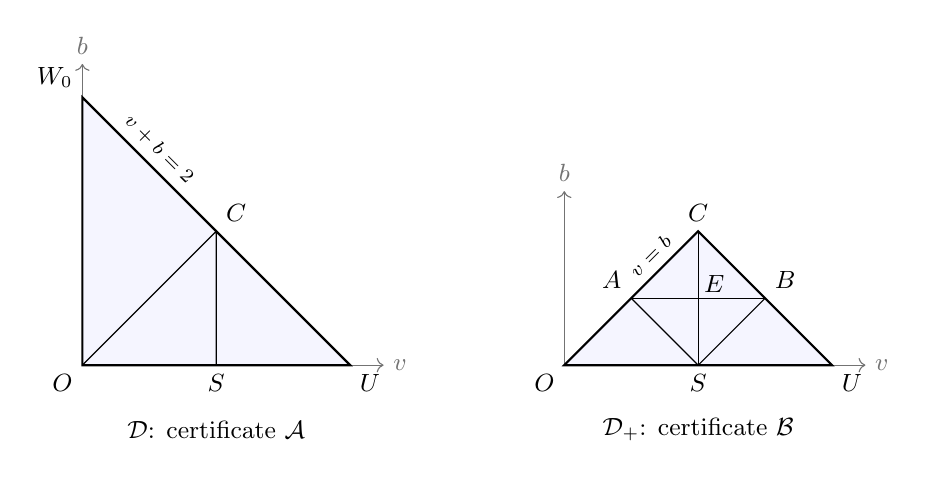
\begin{tikzpicture}[scale=1.7, every node/.style={font=\small}]
 \begin{scope}
  \fill[blue!4] (0,0)--(2,0)--(0,2)--cycle;
  \draw[->,black!55] (0,0)--(2.25,0) node[right] {$v$};
  \draw[->,black!55] (0,0)--(0,2.25) node[above] {$b$};
  \draw[thick] (0,0)--(2,0)--(0,2)--cycle;
  \path (2,0)--(0,2) node[pos=.76,above,sloped,font=\scriptsize]
    {$v+b=2$};
  \draw (0,0)--(1,1)--(1,0);
  \node[below left] at (0,0) {$O$};
  \node[below] at (1,0) {$S$};
  \node[below right] at (2,0) {$U$};
  \node[above right] at (1,1) {$C$};
  \node[above left] at (0,2) {$W_0$};
  \node at (1,-0.48) {$\mathcal D$: certificate $\mathcal A$};
 \end{scope}
 \begin{scope}[xshift=3.6cm]
  \fill[blue!4] (0,0)--(2,0)--(1,1)--cycle;
  \draw[->,black!55] (0,0)--(2.25,0) node[right] {$v$};
  \draw[->,black!55] (0,0)--(0,1.3) node[above] {$b$};
  \draw[thick] (0,0)--(2,0)--(1,1)--cycle;
  \path (0,0)--(1,1) node[pos=.73,above,sloped,font=\scriptsize]
    {$v=b$};
  \draw (0.5,0.5)--(1,0)--(1.5,0.5);
  \draw (1,0)--(1,1);
  \draw (0.5,0.5)--(1.5,0.5);
  \node[below left] at (0,0) {$O$};
  \node[below] at (1,0) {$S$};
  \node[below right] at (2,0) {$U$};
  \node[above] at (1,1) {$C$};
  \node[above left] at (0.5,0.5) {$A$};
  \node[above right] at (1.5,0.5) {$B$};
  \node[above right,inner sep=2pt] at (1,0.5) {$E$};
  \node at (1,-0.48) {$\mathcal D_+$: certificate $\mathcal B$};
 \end{scope}
\end{tikzpicture}
\caption{Subdivisions of the Weyl-norm domains
$\mathcal D=\{(v,b):v,b\ge0,\ v+b\le2\}$ and
$\mathcal D_+=\mathcal D\cap\{v\ge b\}$ used in the triangular
coefficient table. Every edge is included. The norm condition
$v+b\le2$ is a necessary relaxation of the sectional-curvature condition;
the tensor estimates retain the stronger constraint $x+y\le2$.}
\label{fig:certificate-domains}
\end{figure}


For a matrix row, the last two columns below bound, respectively,
\[
 \min([r]_{ij},[h']_{ij}),\qquad
 [r]_{ij}[h']_{ij}-[s']_{ij}^{2}.
\]
Thus the last column is the determinant of each coefficient matrix.
For a scalar row, the first bound applies directly to its coefficient.
The bounds apply to every nonzero coefficient; a zero matrix exception
means that all three of its entries vanish.
\begin{center}
\small
\begin{tabular}{@{}lcccrr@{}}
\toprule
Object & Triangle & $N$ & Zeros &
 \shortstack{Diagonal or\\scalar bound} & Determinant bound\\
\midrule
$\mathcal A$ & $OSC$ & $8$ & $0$ & $16000$ & $53000000$\\
 & $OCW_0$ & $8$ & $0$ & $890$ & $3900000$\\
 & $SCU$ & $8$ & $0$ & $2400$ & $3500000$\\
\midrule
$\mathcal B$ & $OAS$ & $9$ & $0$ & $43$ & $1050$\\
 & $ASE$ & $9$ & $0$ & $43$ & $490$\\
 & $ACE$ & $10$ & $1$ & $2$ & $21$\\
 & $SBE$ & $9$ & $0$ & $43$ & $1300$\\
 & $CBE$ & $10$ & $2$ & $13/100$ & $4$\\
 & $SUB$ & $9$ & $0$ & $5$ & $290$\\
\midrule
$L_v$ & $OCU$ & $6$ & $1$ & $9/10$ & ---\\
$F+12c\delta^2L_b$ & $OSC$ & $9$ & $6$ & $19/100$ & ---\\
 & $SCU$ & $9$ & $7$ & $9/1000$ & ---\\
\bottomrule
\end{tabular}
\end{center}

Here are explicit expansion instructions for all entries of the table.
They also fix the coefficient ordering. Write
$a=V-1$, $s=W-1$ in \eqref{eq:15} and form $\kappa(V,W)$ and
its two partial derivatives. A partial derivative is obtained by
reducing the appropriate exponent of each monomial and multiplying by
that exponent. Differentiate before substituting the affine expressions
$V,W$. Put
\[
 \kappa_* =\kappa(V,W),\qquad \bar\kappa_* =\kappa(W,V).
\]
Thus the partial derivatives of the exchanged function, before affine
substitution, are
\[
 \partial_V\bar\kappa_*(V,W)=(\partial_2\kappa)(W,V),\qquad
 \partial_W\bar\kappa_*(V,W)=(\partial_1\kappa)(W,V).
\]

Ordinary coefficient arrays are multiplied by convolution:
\[
 (PQ)_{de}=\sum_{f=0}^d\sum_{g=0}^e P_{fg}Q_{d-f,e-g}.
\]
Use
\[
\begin{aligned}
 m_*&=\left(1-\frac38(V-W)\right)^2,
       &d_0&=2-V-W,\\
 P_{k,*}&=300m_*+160h d_0,
       &P_{l,*}&=35m_*V,\\
 Y_*&=m_*(42+3W^2+10V^2)
       -h\bigl[6(V^2+W^2-V-W)-26d_0\bigr].
\end{aligned}
\]
For $\mathcal A$, apply $s_{ij}$ from
Lemma~\ref{lem:bernstein-conversion} to the three entries of
\[
\begin{aligned}
 &(P_{k,*}+30hV)
       \bigl\{V(A_1,Y_*,A_{12})-\kappa_*(5,1,0)\bigr\}\\
 &\hspace{22mm}-2V^2(P_{k,*}^2,P_{l,*}^2,P_{k,*}P_{l,*}),
\end{aligned}
\]
where
\[
 A_1=5Y_*+m_*(300V+140V^2)+160h d_0V,
 \qquad
 A_{12}=m_*(75V+35V^2)+40h d_0V.
\]
These are the original entries of \eqref{eq:21} at $\sigma=1$, expressed
only in the affine polynomials $V,W$.

For $\mathcal B$, put
\[
\begin{aligned}
 K_*&=4+V^2+W^2,\qquad \Theta_* =\Theta(V,W),\\
 X_*&=m_*(-70+100V-25V^2-5W^2)
       +\frac53h\bigl(6(a^2+s^2)+32a d_0\bigr),\\
 H_*&=8VK_*\Theta_*(1+V)\\
 &\quad-(1+6V+V^2)
       \left\{VD+K_*\left[V\bigl(X_*+(\partial_1\kappa)(V,W)\bigr)
                                     +\frac{2\kappa_*}{3}\right]\right\}.
\end{aligned}
\]
Apply $s_{ij}$ to $H_*$, to its exchange in $V,W$, and to
\[
 S_*(V,W)\left\{
       \frac{K_*}{2}\bigl((\partial_2\kappa)(V,W)
                        +(\partial_2\kappa)(W,V)\bigr)-D\right\}.
\]
For example, on $CBE$ the triples at $(i,j)=(8,0),(8,1),(8,2)$ are
\[
 \left(\frac{11041}{810},\frac{4063}{810},\frac{60557}{16200}\right),
 \quad
 \left(\frac{4328}{405},\frac{839}{405},\frac{3977}{2700}\right),
 \quad
 \left(\frac{191}{81},\frac{191}{81},-\frac{1189}{1350}\right).
\]

For the two scalar rows, apply $s_{ij}$ to
$10h d_0V-\kappa_*$ and, respectively, to
\[
\begin{aligned}
 c(V,W)\bigg\{&D\left(1-\frac{d_0^2}{4}\right)(V-W)^2
       +30h d_0(V^2a^2+W^2s^2)\\
 &+6(Va\kappa_*+Ws\bar\kappa_*)
       +12d_0^2(10h d_0W-\bar\kappa_*)\bigg\}-\Theta_*^2.
\end{aligned}
\]
Together with the coefficient-sum formula, these prescriptions produce
the displayed rational bounds by addition and multiplication of finite
arrays.

The zero exceptions are as follows, with the third homogeneous index
always $N-i-j$. For $\mathcal B$, they are the vertex $C$ in $ACE$
and $CBE$, namely $(0,10,0)$ and $(10,0,0)$, and also $(9,1,0)$ in
$CBE$. For $L_v$ the only zero is $(0,6,0)$, the vertex $C$ in $OCU$.
For $F+12c\delta^2L_b$ on $OSC$, the zeros are exactly $i+j\le2$.
On $SCU$ they are exactly $9-j\le2$, together with $(i,j)=(0,6)$.
There are no other exceptions.

Every nonzero matrix coefficient has positive diagonal entries and
positive determinant, and each exceptional matrix is zero. Thus all
coefficient matrices are positive semidefinite. The scalar coefficients
are all nonnegative. Lemma~\ref{lem:bernstein-conversion} and the stated
domain coverage prove the assertions.
\end{proof}

\subsection{The remaining potential polynomial}

\begin{lemma}[The polynomial $F$]\label{lem:potential-certificate}
The polynomial $F=cE_0-\Theta^2$ is nonnegative on $\mathcal D$.
\end{lemma}

\begin{proof}
Use $v=1-n+t$, $b=1-n-t$. The full domain becomes
\[
 0\le n\le1,\qquad |t|\le1-n.
\]
Write $F_*(n,t)=F(1-n+t,1-n-t)$ for the pullback to these coordinates.
It is even in $t$, and direct expansion gives
$F_*=\sum_{j=0}^4 f_j(n)t^{2j}$, where
\[
\begin{aligned}
 240f_0={}&n^3(1-n)\bigl(53511n^4-151593n^3
                 +222537n^2-83607n+10256\bigr),\\
 60f_1={}&n\bigl(19389n^5-418926n^4+523719n^3
                 -289776n^2+67782n+10564\bigr),\\
 60f_2={}&-1260129n^4+1370598n^3-451164n^2+23442n+74,\\
 10f_3={}&-12200n^2+2601n+75,\qquad
 f_4=-\frac{23}{5}.
\end{aligned}
\]
For $n<1$, put $z=t^2/(1-n)^2\in[0,1]$. The degree-four Bernstein
coefficients in $z$ are
\[
 h_i(n)=\sum_{j=0}^i
       \frac{\binom ij}{\binom4j}f_j(n)(1-n)^{2j},
 \qquad 0\le i\le4.
\]
Define
\[
 d_0(n)=n^3(1-n),\qquad d_1(n)=n(1-n),\qquad
 d_2(n)=d_3(n)=d_4(n)=1-n.
\]
Each quotient $q_i=h_i/d_i$ is a polynomial. Applying the interval
conversion formula to it on each of the four intervals
\[
 [0,1/4],\quad[1/4,1/2],\quad[1/2,3/4],\quad[3/4,1]
\]
gives the following lower bounds for every coefficient:
\begin{center}
\begin{tabular}{@{}cccc@{}}
\toprule
$i$ & Divisor $d_i$ & Degree of $q_i$ & Lower bound\\
\midrule
$0$ & $n^3(1-n)$ & $4$ & $3$\\
$1$ & $n(1-n)$ & $6$ & $31$\\
$2$ & $1-n$ & $7$ & $1/5$\\
$3$ & $1-n$ & $7$ & $12/5$\\
$4$ & $1-n$ & $7$ & $9/5$\\
\bottomrule
\end{tabular}
\end{center}
The complete prescription for each entry is to insert the displayed
$f_j$ into $h_i$, cancel the indicated polynomial factor, and apply
the coefficient sum in Lemma~\ref{lem:bernstein-conversion} in the
listed degree. In particular, the identities $h_i=d_iq_i$ hold as
polynomial identities, including at the endpoints.

Since every $d_i$ is nonnegative on $[0,1]$, every $h_i$ is
nonnegative. Therefore
\[
 F_*=\sum_{i=0}^4h_i(n)\binom4i z^i(1-z)^{4-i}\ge0
 \qquad(n<1).
\]
At $n=0$, the coordinate $z=t^2$ still covers the entire permitted
interval $|t|\le1$; the vanishing of $h_0,h_1$ causes no difficulty.
At $n=1$, the domain contains only $t=0$, and directly
$F_*(1,0)=F(0,0)=f_0(1)=0$. Thus no numerical division by a vanishing factor
is required, and all of $\mathcal D$ is covered.
\end{proof}

Lemmas~\ref{lem:scalar-certificates}, \ref{lem:matrix-certificates},
and \ref{lem:potential-certificate} establish every polynomial
inequality used in Section~\ref{sec:coupling}. Hence the three estimates
of Proposition~\ref{prop:coupling-estimates} hold on the stated
positive-variable spectral domain. The compatible limit in
Section~\ref{sec:coupling} extends them to the zero sets under the
nonnegative sectional-curvature hypothesis.

\clearpage
\begin{thebibliography}{99}
\raggedright
\addcontentsline{toc}{section}{\refname}

\bibitem{Berger1961}
M.~Berger, \emph{Sur quelques vari\'et\'es d'Einstein compactes}, Ann. Mat. Pura Appl. \textbf{53} (1961), 89--95.
\href{https://doi.org/10.1007/BF02417787}{doi:10.1007/BF02417787}.

\bibitem{BoudaoudCarusoRoy2008}
F.~Boudaoud, F.~Caruso, and M.-F.~Roy, \emph{Certificates of Positivity in the Bernstein Basis}, Discrete Comput. Geom. \textbf{39} (2008), no.~4, 639--655.
\href{https://doi.org/10.1007/s00454-007-9042-x}{doi:10.1007/s00454-007-9042-x}.

\bibitem{Brendle2010}
S.~Brendle, \emph{Einstein manifolds with nonnegative isotropic curvature are locally symmetric}, Duke Math. J. \textbf{151} (2010), no.~1, 1--21.
\href{https://doi.org/10.1215/00127094-2009-061}{doi:10.1215/00127094-2009-061}.

\bibitem{CalderbankGauduchonHerzlich2000}
D.~M.~J.~Calderbank, P.~Gauduchon, and M.~Herzlich, \emph{Refined Kato inequalities and conformal weights in Riemannian geometry}, J. Funct. Anal. \textbf{173} (2000), no.~1, 214--255.
\href{https://doi.org/10.1006/jfan.2000.3563}{doi:10.1006/jfan.2000.3563}.

\bibitem{CaoTran2018}
X.~Cao and H.~Tran, \emph{Einstein four-manifolds of pinched sectional curvature}, Adv. Math. \textbf{335} (2018), 322--342.
\href{https://doi.org/10.1016/j.aim.2018.07.003}{doi:10.1016/j.aim.2018.07.003}.
Author version: \href{https://arxiv.org/abs/1612.06023v2}{arXiv:1612.06023v2}.

\bibitem{Cheng2026}
L.~Cheng, \emph{On Positively Curved Einstein Four-Manifolds with Euler Characteristic at Most Three}, \href{https://arxiv.org/abs/2609.23337v1}{arXiv:2609.23337v1} [math.DG], September 20, 2026.

\bibitem{Costa2004}
E.~Costa, \emph{On Einstein four-manifolds}, J. Geom. Phys. \textbf{51} (2004), no.~2, 244--255.
\href{https://doi.org/10.1016/j.geomphys.2003.10.013}{doi:10.1016/j.geomphys.2003.10.013}.

\bibitem{Derdzinski1983}
A.~Derdzi\'nski, \emph{Self-dual K\"ahler manifolds and Einstein manifolds of dimension four}, Compositio Math. \textbf{49} (1983), no.~3, 405--433. \href{https://www.numdam.org/item/CM_1983__49_3_405_0/}{Journal archive}.

\bibitem{deRham1952}
G.~de~Rham, \emph{Sur la r\'eductibilit\'e d'un espace de Riemann},
Comment. Math. Helv. \textbf{26} (1952), 328--344.
\href{https://doi.org/10.1007/BF02564308}{doi:10.1007/BF02564308}.

\bibitem{DiCerbo2026}
L.~F.~Di Cerbo, \emph{A rigidity theorem for Einstein 4-manifolds with sectional curvature of a fixed sign, and its consequences}, Math. Ann. \textbf{396} (2026), article 11.
\href{https://doi.org/10.1007/s00208-026-03547-w}{doi:10.1007/s00208-026-03547-w}.
Author version: \href{https://arxiv.org/abs/2503.09570v3}{arXiv:2503.09570v3}.

\bibitem{Gilkey1984}
P.~B.~Gilkey, \emph{Invariance Theory, the Heat Equation, and the Atiyah--Singer Index Theorem}, Publish or Perish, 1984. \href{https://pages.uoregon.edu/gilkey/dirPDF/InvarianceTheory1Ed.pdf}{Author-hosted electronic reprint, 1996}.

\bibitem{GurskyLeBrun1999}
M.~J.~Gursky and C.~LeBrun, \emph{On Einstein manifolds of positive sectional curvature}, Ann. Global Anal. Geom. \textbf{17} (1999), no.~4, 315--328.
\href{https://doi.org/10.1023/A:1006597912184}{doi:10.1023/A:1006597912184}.

\bibitem{GurskyMalchiodi2026}
M.~J.~Gursky and A.~Malchiodi,
\emph{Einstein four-manifolds of positive sectional curvature and ADM mass},
\href{https://arxiv.org/abs/2609.30803v1}{arXiv:2609.30803v1} [math.DG], submitted September 25, 2026.

\bibitem{Hitchin1981}
N.~J.~Hitchin, \emph{K\"ahlerian twistor spaces},
Proc. London Math. Soc. (3) \textbf{43} (1981), no.~1, 133--150.
\href{https://doi.org/10.1112/plms/s3-43.1.133}{doi:10.1112/plms/s3-43.1.133}.

\bibitem{Ilias}
S.~Ilias, \emph{Constantes explicites pour les in\'egalit\'es de Sobolev sur les vari\'et\'es riemanniennes compactes}, Ann. Inst. Fourier (Grenoble) \textbf{33} (1983), no.~2, 151--165.
\href{https://doi.org/10.5802/aif.921}{doi:10.5802/aif.921}.

\bibitem{Liu2025}
T.~Liu, \emph{Toric Einstein 4-manifolds with non-negative sectional curvature},
Ann. Global Anal. Geom. \textbf{67} (2025), article 14.
\href{https://doi.org/10.1007/s10455-025-09990-3}{doi:10.1007/s10455-025-09990-3}.

\bibitem{MicallefWang1993}
M.~J.~Micallef and M.~Y.~Wang,
\emph{Metrics with nonnegative isotropic curvature},
Duke Math. J. \textbf{72} (1993), no.~3, 649--672.
\href{https://doi.org/10.1215/S0012-7094-93-07224-9}{doi:10.1215/S0012-7094-93-07224-9}.

\bibitem{Myers1941}
S.~B.~Myers, \emph{Riemannian manifolds with positive mean curvature}, Duke Math. J. \textbf{8} (1941), no.~2, 401--404.
\href{https://doi.org/10.1215/S0012-7094-41-00832-3}{doi:10.1215/S0012-7094-41-00832-3}.

\bibitem{Obata1962}
M.~Obata, \emph{Certain conditions for a Riemannian manifold to be isometric with a sphere},
J. Math. Soc. Japan \textbf{14} (1962), no.~3, 333--340.
\href{https://doi.org/10.2969/jmsj/01430333}{doi:10.2969/jmsj/01430333}.

\bibitem{OpenAI2026P}
OpenAI, \emph{Positively curved Einstein four-manifolds},
OpenAI Math Release preprint
\href{https://github.com/openai/math/blob/main/preprints/Positively-curved-Einstein-four-manifolds-September-23-2026/paper.pdf}{OAI:Positively-curved-Einstein-four-manifolds-September-23-2026},
2026.

\bibitem{Roy2007}
M.-F.~Roy, \emph{Certificates of Positivity in the Bernstein basis}, Oberwolfach Reports, report 14/2007, 800--804. Report on joint work with F.~Boudaoud, F.~Caruso, and R.~Leroy. \href{https://ems.press/content/serial-article-files/46100}{Report}.

\bibitem{Yang2000}
D.~Yang, \emph{Rigidity of Einstein 4-manifolds with positive curvature}, Invent. Math. \textbf{142} (2000), no.~2, 435--450.
\href{https://doi.org/10.1007/PL00005792}{doi:10.1007/PL00005792}.

\end{thebibliography}

\end{document}
